\documentclass[12pt]{article}
\usepackage{bookmark}
\usepackage{graphicx}
\usepackage[a4paper]{geometry}
\usepackage{amsmath}
\usepackage{amssymb}
\usepackage{float}
\begin{document}
\title{Notes on Single Variable Calculus}
\author{BatuCem}
\maketitle
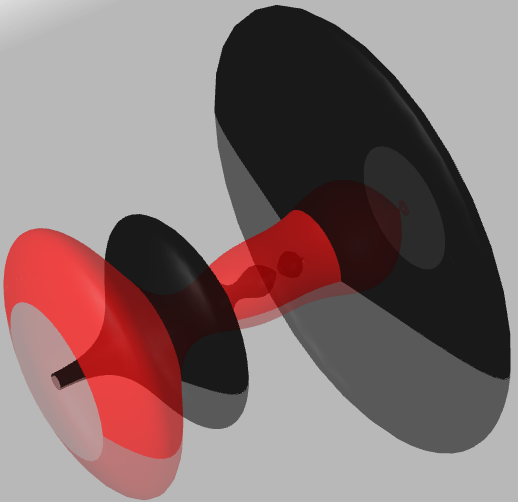
\includegraphics[scale=1]{A.png}

\begin{small}
The main purpose of these notes is to briefly remind the contents of it to those who already learnt them and to make a collection of the single variable calculus subjects without going into too much detail.
\end{small}
\newpage
\tableofcontents
\newpage
\section{Limits and Continuity}
\subsection{Defining Limits}
\textbf{Intuitive (Informal) definition of limits}: If $f(x)$ is defined for all $x$ near $a$, except possibly at $a$ itself, and if we can
ensure that $f(x)$ is as close as we want to $L$ by taking $x$ close enough to $a$,
but not equal to $a$, we say that the function $f$ approaches the limit $L$ as $x$
approaches $a$, and we write $$\lim \limits_{x \to a} f(x)=L$$

\textbf{Formal definition of limits}: We say that $f(x)$ approaches the limit $L$ as $x$ approaches $a$, and we write $$\lim \limits_{x \to a} f(x)=L$$ if the following condition is satisfied:\\
For every number $\epsilon > 0$ there exists a number $\delta > 0$, possibly depending on $\epsilon$ , such that if $0<|x-a|<\delta$, then $x$ belongs to the domain of $f$ and $|f(x)-L|<\epsilon$. Often summarized in form $$(\forall \epsilon > 0 )(\exists \delta > 0), |x-a|<\delta \Rightarrow |f(x)-L|<\epsilon$$

Similar statement is made for limits where either $x \to \mp \infty$ or $L= \mp \infty$: 
$$\lim \limits_{x \to \infty} f(x)=L \Leftrightarrow (\forall \epsilon > 0 )(\exists N > 0), x>N \Rightarrow |f(x)-L|<\epsilon$$

$$\lim \limits_{x \to -\infty} f(x)=L \Leftrightarrow (\forall \epsilon > 0 )(\exists N < 0), x<N \Rightarrow |f(x)-L|<\epsilon$$

$$\lim \limits_{x \to a} f(x)=\infty  \Leftrightarrow (\forall K>0 )(\exists \delta > 0), |x-a|<\delta \Rightarrow f(x)>K$$

$$\lim \limits_{x \to a} f(x)=-\infty  \Leftrightarrow (\forall K<0 )(\exists \delta > 0), |x-a|<\delta \Rightarrow f(x)<K$$
%\newpage
%Personal Note: It must be seen that the formal definition of limit is cumbersome yet it is the only way to properly prove that a limit exists for an expression. It is to me, after a year of dealing with calculus, still the single hardest thing in calculus, single or multivariable. It is usually better to do the comparisons as much as it is, and be done with it since the problems it arises are confusing and if you wanted to abuse the definition you can possibly prove that $\lim \limits_{x \to 5} x = 3$ or any number really. The important thing here is that in single variable calculus, we have two possible ways of proving a limits existence and its value, one is the usage of the formal definition and the other is approaching the function from the right-hand side and from the left-hand side, however the approach method will not work in multivariable limits and we will have to use the formal definition to prove all and any multivariable function limits.

The powers of limits are that we can approach and learn about the behaviour of a function at a point even if such point is undefined on said function and that we can see the behaviour of a function at $x \to \infty$ or $x \to -\infty$.

\newpage
\textbf{One very important limit:} $$\lim \limits_{x \to \infty} \left(1+\frac{1}{x}\right)^x= e$$

\textbf{Example}: Using $\epsilon -\delta$ definition, show that the $\lim \limits_{x \to 2} x^2=4$.

\textbf{Solution}: $$\left(|x^2-4|= |x-2|\cdot |x+2|<\epsilon \Rightarrow |x-2|<\dfrac{\epsilon}{|x+2|}\right) \ \ \wedge \ \ $$$$\left(|x-2|<\delta<1 \Rightarrow 3<x+2<5 \Rightarrow \frac{1}{5}<\frac{1}{|x+2|}<\frac{1}{3}\right)$$$$\Rightarrow \left(\delta \leq \frac{\epsilon}{5} \Rightarrow |x-2|<\delta\leq \frac{\epsilon}{5}\right)$$$$\Rightarrow |x^2-4|<|x+2|\cdot \frac{\epsilon}{5}<|x+2| \frac{\epsilon}{|x+2|} = \epsilon.$$
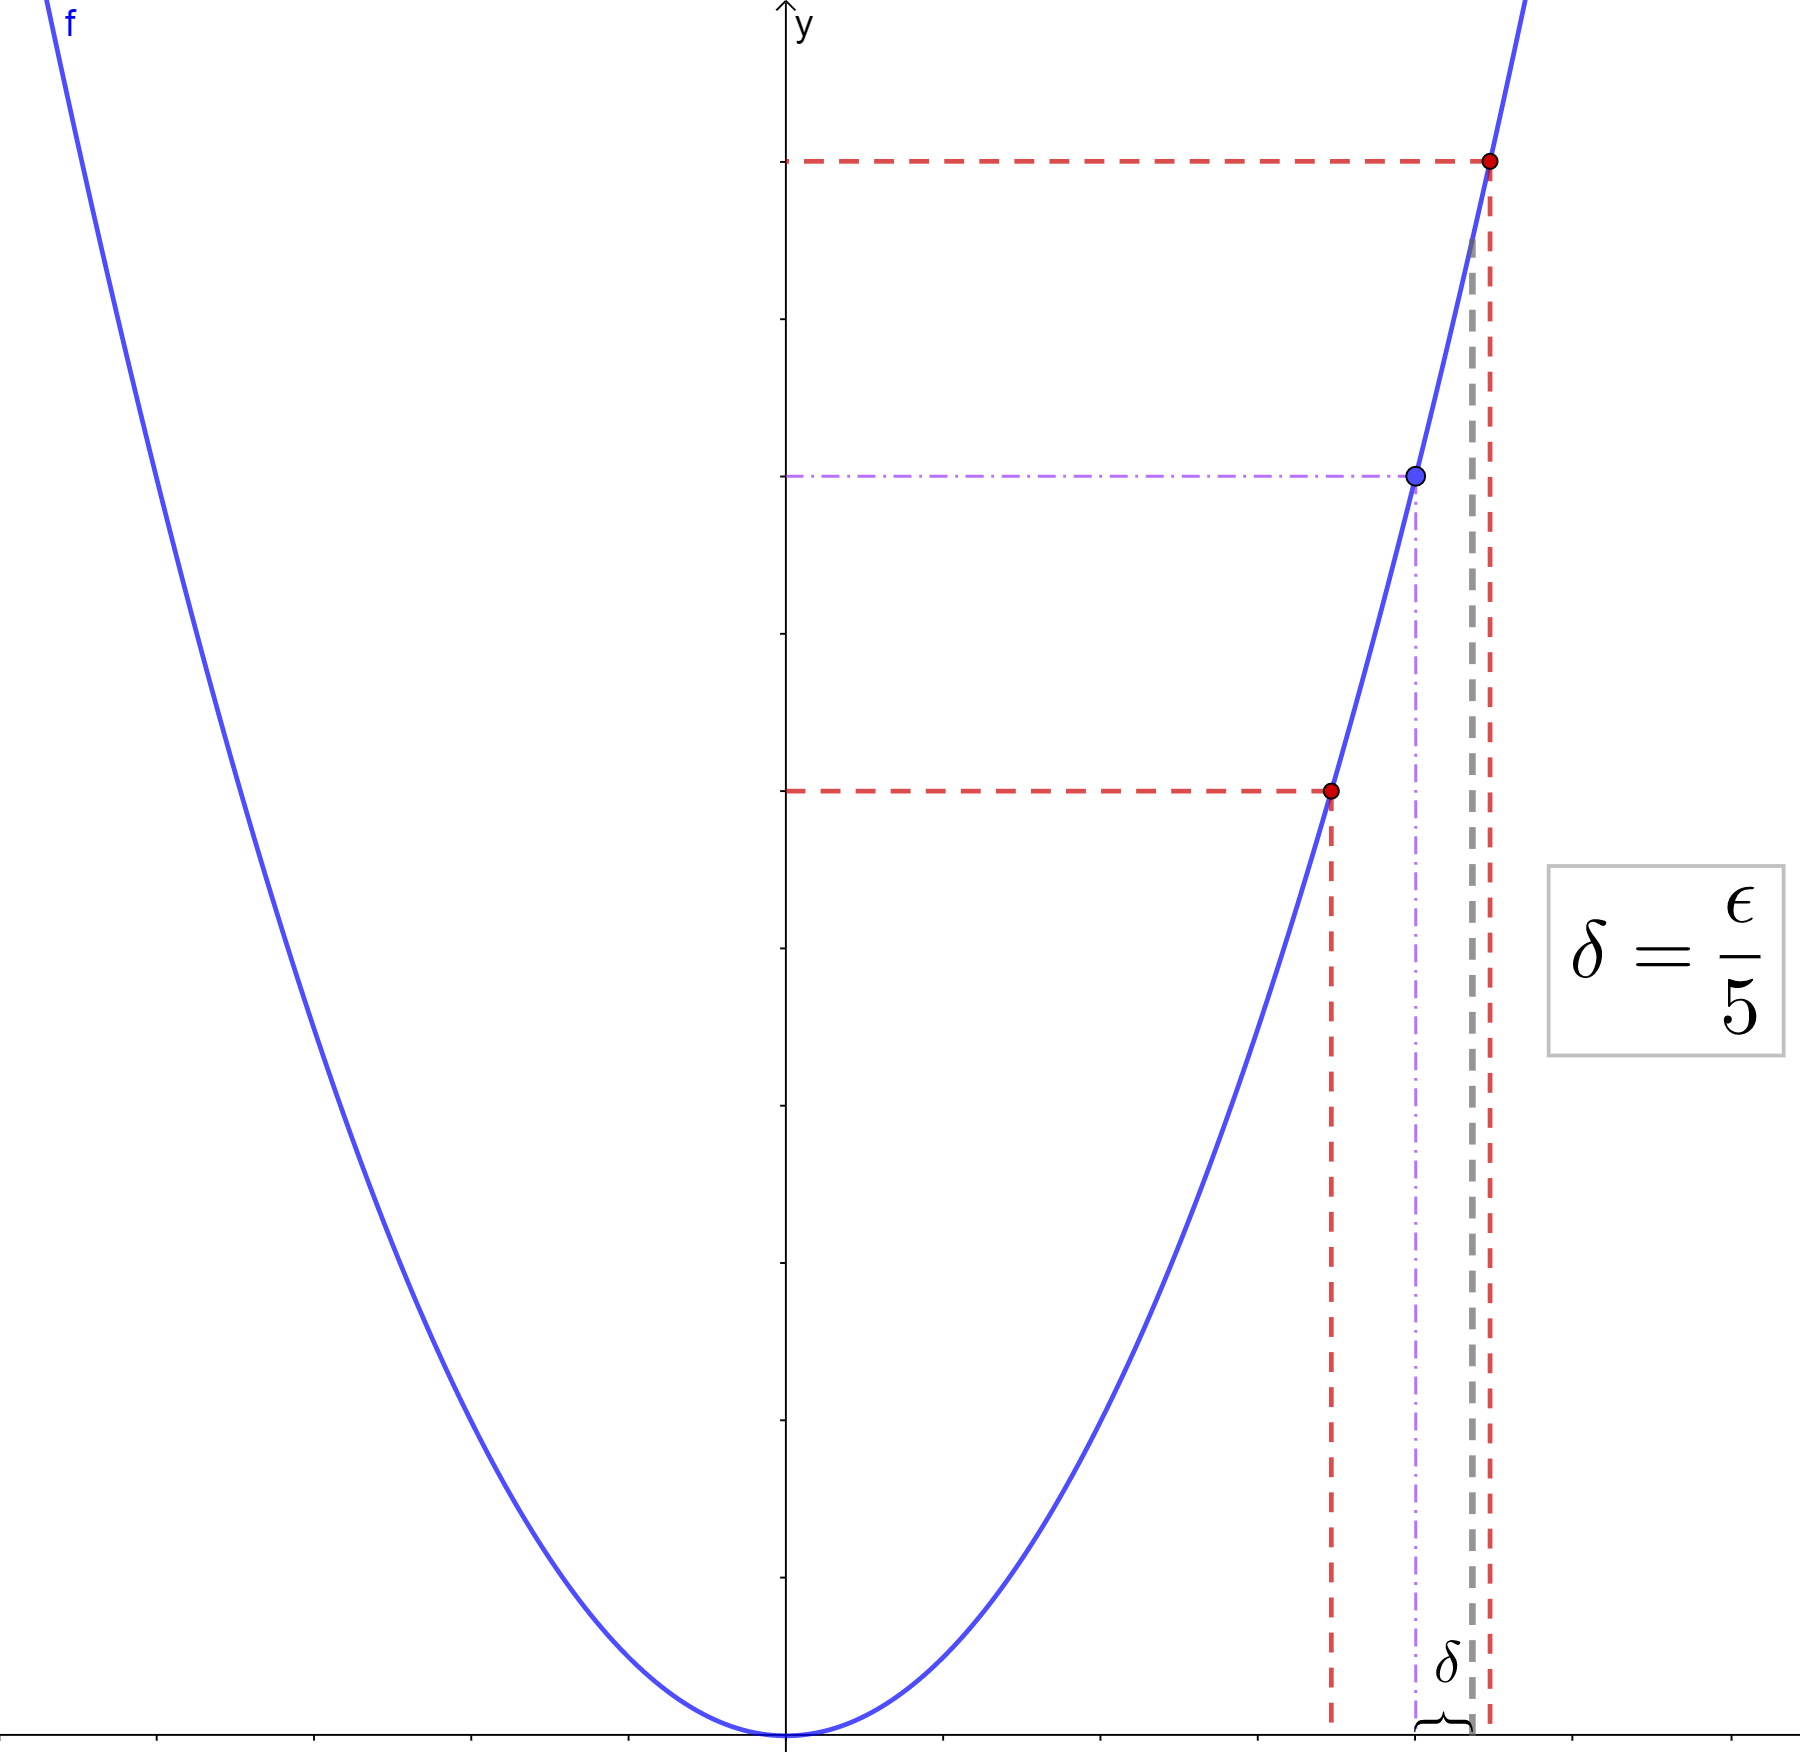
\includegraphics[scale=0.28]{epsilondelta.png}
\newpage
\subsection{Squeeze Theorem}
The squeeze theorem states that if we had three functions $f(x),\ g(x),\ h(x)$ such that $f(x)\leq g(x) \leq h(x) \ ,\ \forall x \in$ $I$ where $I$ is possibly an open interval that contains \\ $a\ \wedge \lim \limits_{x \to a} f(x) = \lim \limits_{x \to a} h(x)=L $, then $\lim \limits_{x \to a} g(x)=L $ also.\\
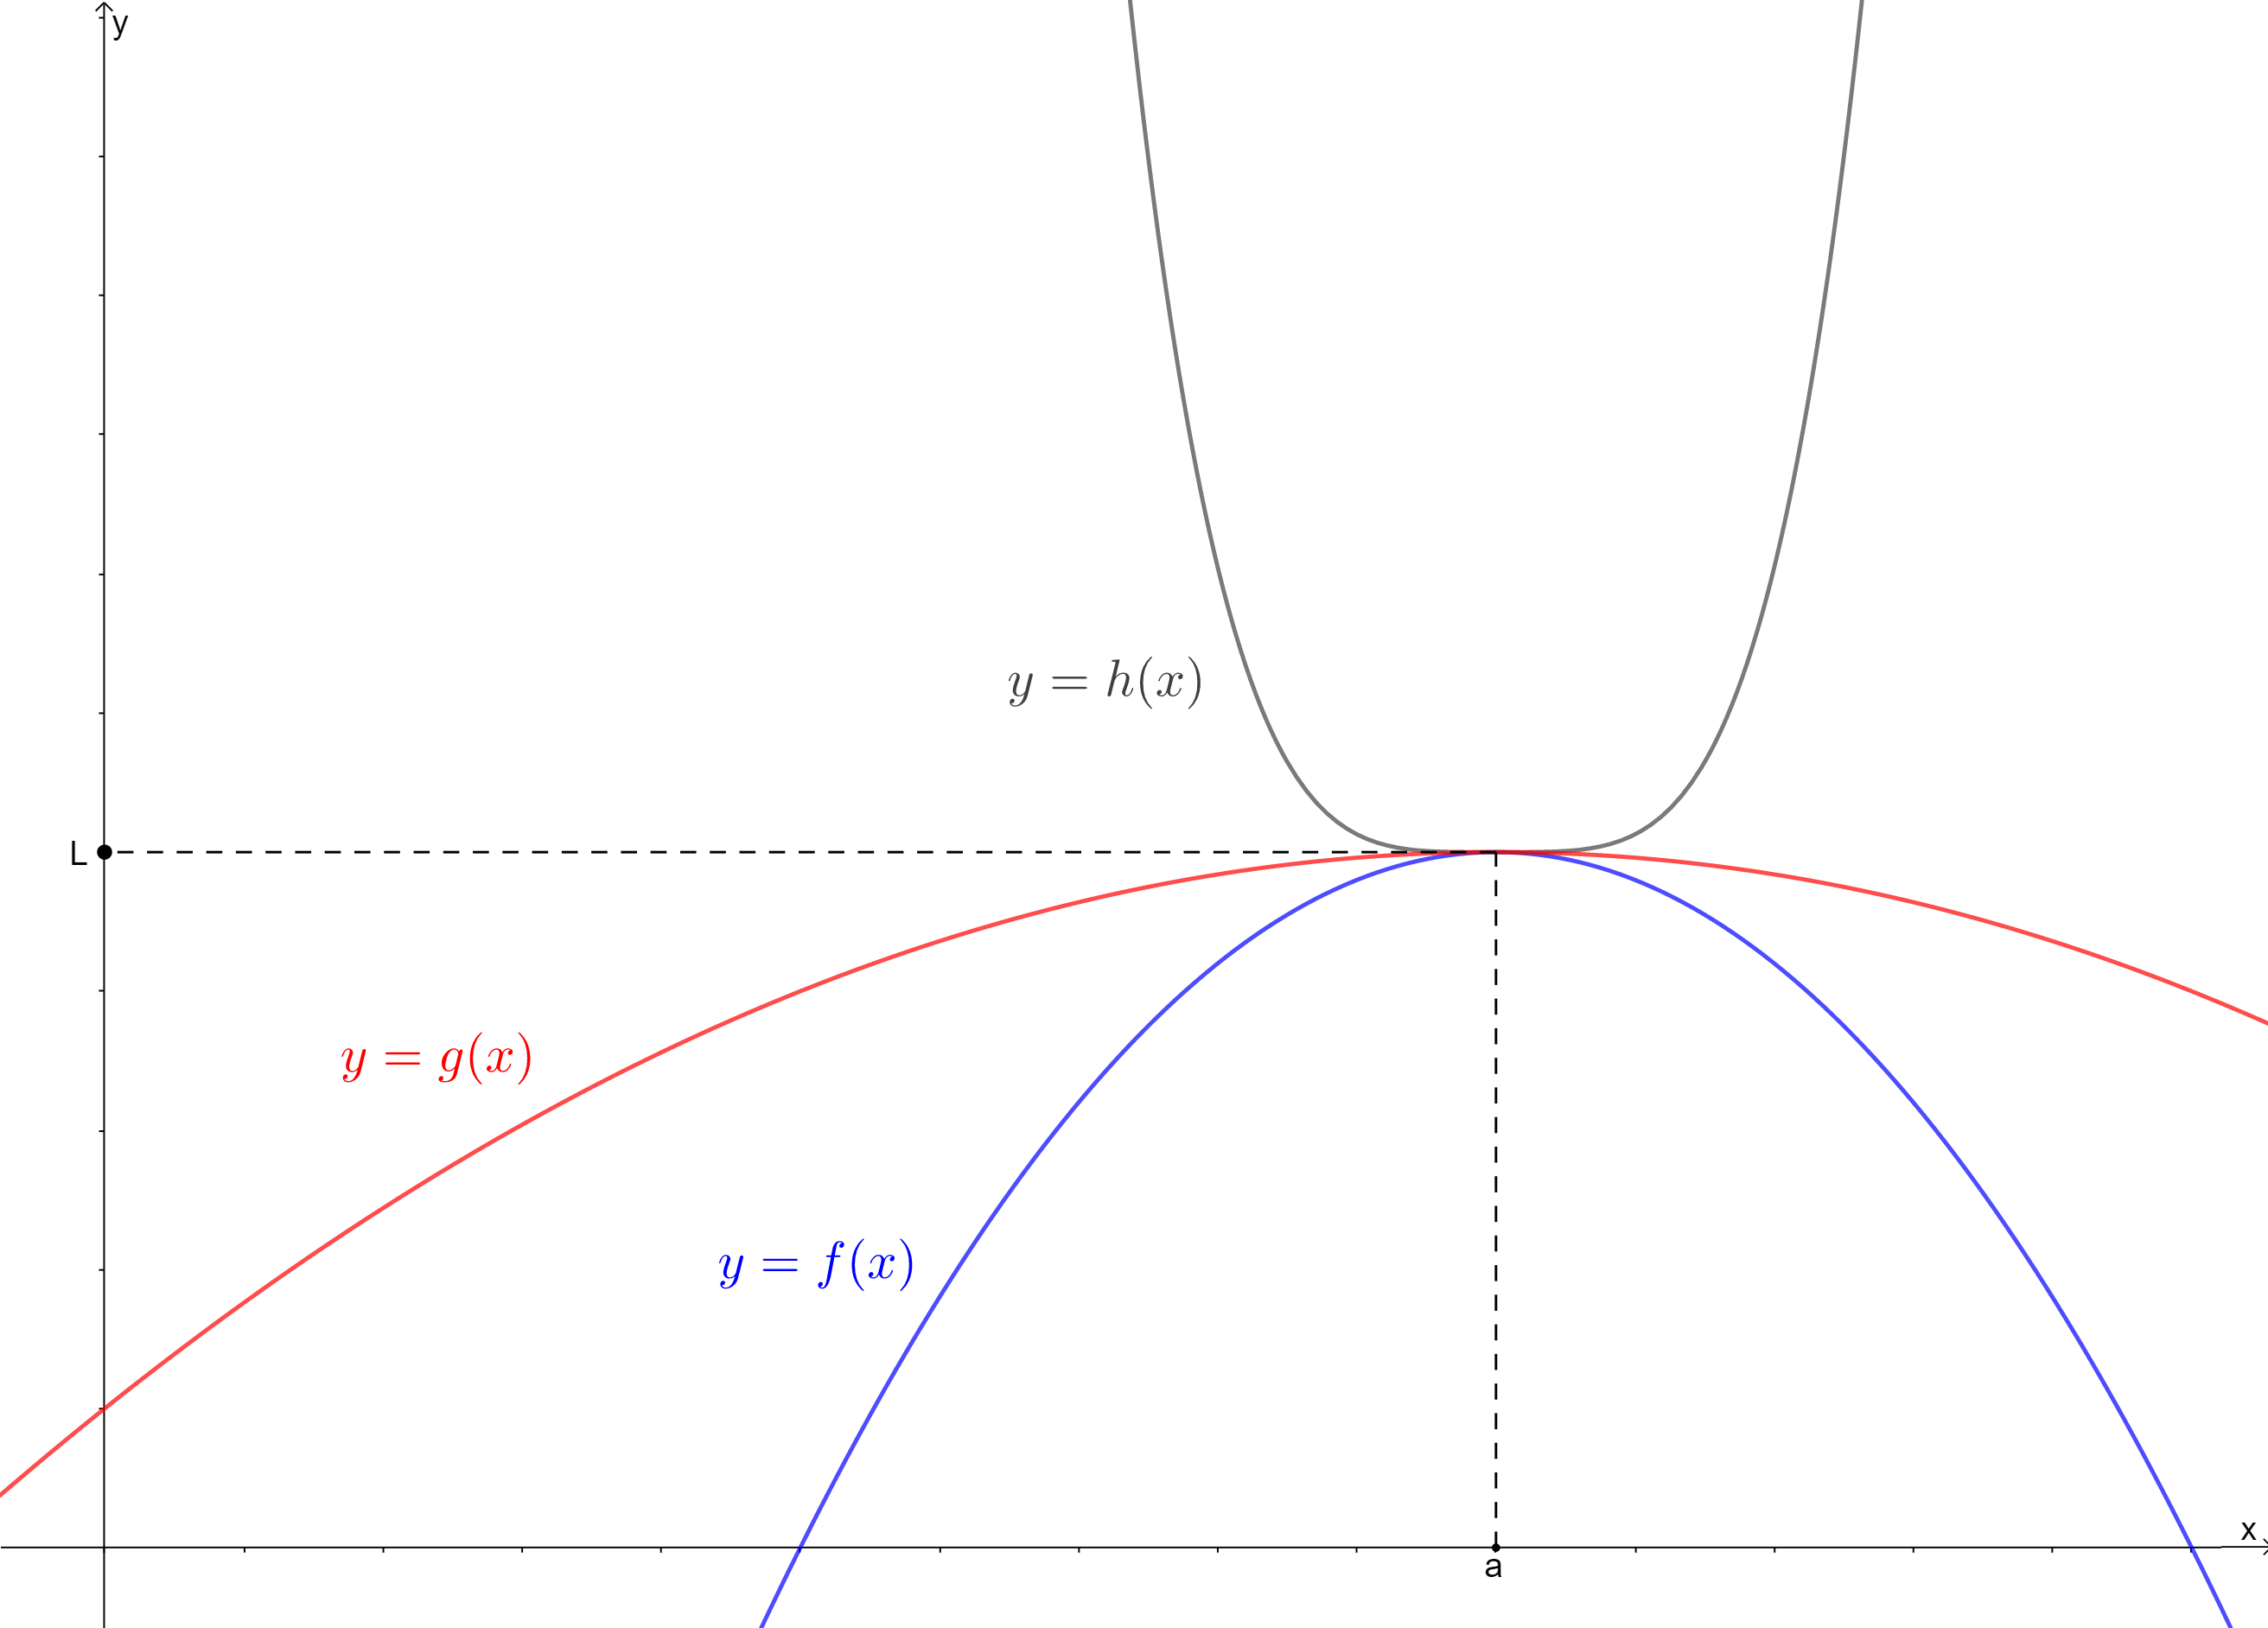
\includegraphics[scale=0.2]{Squeeze.png}
\subsection{Continuity}
Let $D$ be the domain of function $f(x)$ and let $a\in D$. We say that the function $f$ is continuous at point $c$ if $\lim \limits_{x \to c} f(x)= f(c)$. So if the limit of $f$ at point $c$ does not exist or $f$ is undefined at point $c$ the function $f$ is discontinuous at point $c$. Intuitively, when you are drawing the function's graph, if you can pass from point $c$ without lifting your pen, then the function $f$ is continuous at point $c$ and actually, if you can draw any interval of a function without lifting your pen, then it could be said that in this interval, the function is continuous. In the endpoints of the function's domain, it is sufficient to get limits from right or left hand side and compare these one sided limits with the function's value to test continuity.
\newpage
\subsection{Max-Min Theorem}
If $f(x)$ is continuous on the closed, finite interval $[a,b]$, then there exist numbers $p$ and $q$ in $[a,b]$ such that $\forall  x \in [a,b]$, $f(p)\leq f(x)\leq f(q)$. Thus, $f$ has the minimum value $min=f(p)$ and maximum value $max=f(q)$.
\subsection{Intermediate Value Theorem}
If $f(x)$ is continuous on the interval $[a,b]$ and if $s$ is a number between $f(a),f(b)$, then there exists a number c in $[a,b]$ such that $f(c)=s$. In fact, this statement follows from the fact that a continuous function takes all values between its maximum and minimum values in a closed input interval.

Intermediate value theorem could be used to find the roots of a continuous function. It takes one to find values $a,b$ where $f(a)<0$ and $f(b)>0$ and then by the IVT statement, there must exist a point $c$ where $f(c)=0$. Using some programming, some linear -or better, binary- search can be formulated in order to find a function's roots in a pre-specified closed interval. In fact, modern calculators find a root by this method or Newton's Method.\\
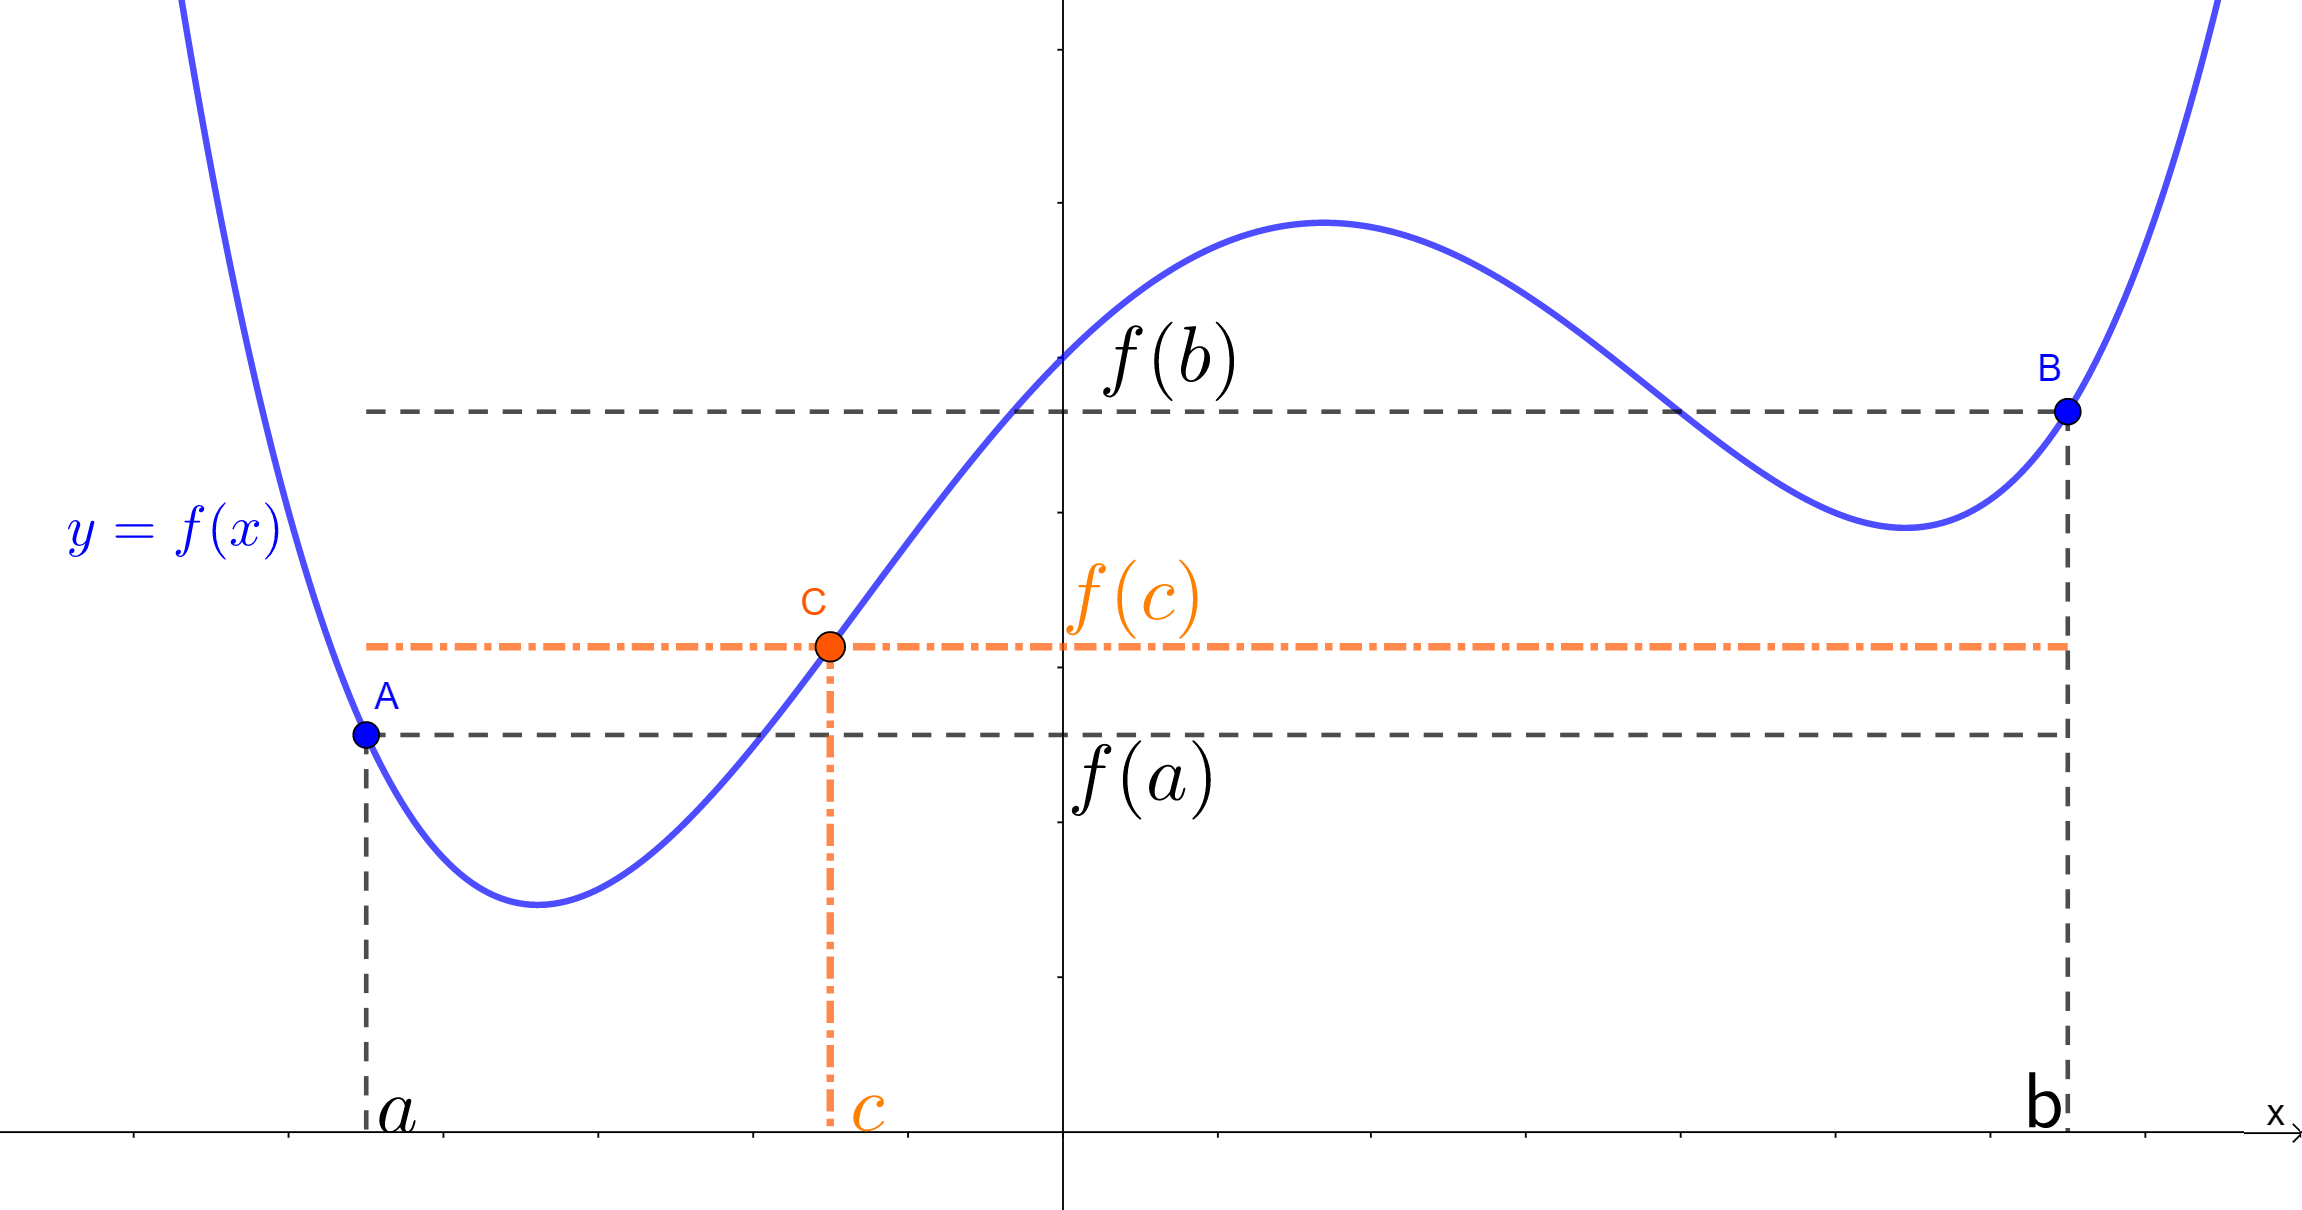
\includegraphics[scale=0.24]{IVT.png}
\section{Differentiation}
\subsection{Defining and Assigning a Meaning to Derivatives and Differentials}
Suppose that we have a continuous function $F(x)$ and we want to find the slope of this at a point, as another function. The first question is that how does one find slope at a point? He does not, at least not directly. We must understand that the limit concept is very important here since if we took two distinct points on $F$ and find the slope of such system, that would not necessarily be the slope of any point, only using the limits we can pick one point at $x_0=c$ and another point $x_1=c+\Delta x$ and we get the slope of these points where $\Delta x \to 0$ and as such, we obtain the derivative function's value at $x=c$. It is useful to note here that $\Delta x \to 0=dx$, $dx$ being called the differential. Also, see that we can not receive a derivative function when we solve numerically. To get a function as a result what was $c$ must be renamed as $x$, as in solving parametrically.\\
As a summary, \textbf{differential} ($dx$): $\Delta x \to 0=dx$.\\
\textbf{Derivative function} $f(x)$:  $\displaystyle{f(x)=\lim \limits_{h \to 0} \frac{F(x+h)-F(x)}{h}}$\\
\textbf{Newton Quotient}: $\displaystyle{\frac{F(x_0+h)-F(x_0)}{h}}$
\subsection{Tangent and Normal Lines}
A tangent line to a function $f(x)$ at point $x_0$ is defined as a linear function $L(x)$ that passes through $f(x_0)$ and has the slope $f'(x_0)$. In this sense,$$ L(x)= f'(x_0)\cdot x+f(x_0)-f'(x_0)\cdot x_0 $$\ \ \ \ 
A normal line can be defined as another linear function $N(x)$ such that $\displaystyle{N'(x)=-\frac{1}{f'(x_0)}}$ and $N(x_0)=f(x_0)$. So $$N(x)=-\frac{x}{f'(x_0)}+f(x_0)+\frac{x_0}{f'(x_0)}$$
\newpage
\subsection{Rules of Differentiation}
\begin{enumerate}
\item If $f$ is differentiable at point $x_0$, then $f$ is continuous on $x_0$.
\item $(f\pm g)'(x)=f'(x)\pm g'(x)$
\item \textbf{The Product Rule}: $(f\cdot g)'(x)=f'(x)\cdot g(x) + f(x)\cdot g'(x)$
\item \textbf{The Reciprocal Rule}: $\displaystyle{ \left( \frac{1}{f} \right) '(x) = -\frac{f'(x)}{f^2(x)}}$ 
\item \textbf{General Power Rule}: $\displaystyle{ \frac{d(x^n)}{dx}= n\cdot x^{n-1}}$
\item \textbf{The Quotient Rule}: $\displaystyle{\left( \frac{f}{g}\right) '(x)=\frac{f'(x)g(x)-g'(x)f(x)}{g^2(x)}}$
\item \textbf{The Chain Rule}: $\displaystyle{\frac{dy}{du}=\frac{dy}{dx} \cdot \frac{dx}{du}}$
\item $\displaystyle{\frac{d(f^{-1}(x))}{dx}=\frac{1}{f'(f^{-1}(x))}}$
\subsection{Derivatives of Elementary Functions}
$\sin '(x)=\cos (x) \\ \cos '(x)=-\sin (x) \\ (e^x)'=e^x \\ \ln '(x)=\frac{1}{x} \\ \tan '(x)=\sec ^2(x) \\ \cot '(x)=-\csc ^2(x) \\ \sec '(x)=\sec (x)\tan (x) \\ \csc '(x)=-\cot (x)\csc (x)\\ \displaystyle{\arccos '(x)=-\frac{1}{\sqrt{1-x^2}}} \\ \displaystyle{\arcsin '(x)=\frac{1}{\sqrt{1-x^2}}} \\ \displaystyle{\arctan '(x)=\frac{1}{1+x^2}}$
\end{enumerate}
\subsection{Mean-Value Theorem}
Suppose that the function $f$ is continuous on the closed, finite interval $[a,b]$ and that
it is differentiable on the open interval $(a,b)$. Then there exists at least one point $c$ in the open interval $(a,b)$ such that $$\frac{f(b)-f(a)}{b-a}=f'(c) .$$ One important special usage of this theorem is when $f(a)=f(b)$, which means that between a and b, there must exist at least one point which is an extremum, If the said function is linear or partially linear, one can say that there is infinite number of extremum points or that there is none. This particular specification of the Mean Value Theorem is said to be Rolle's Theorem.\\
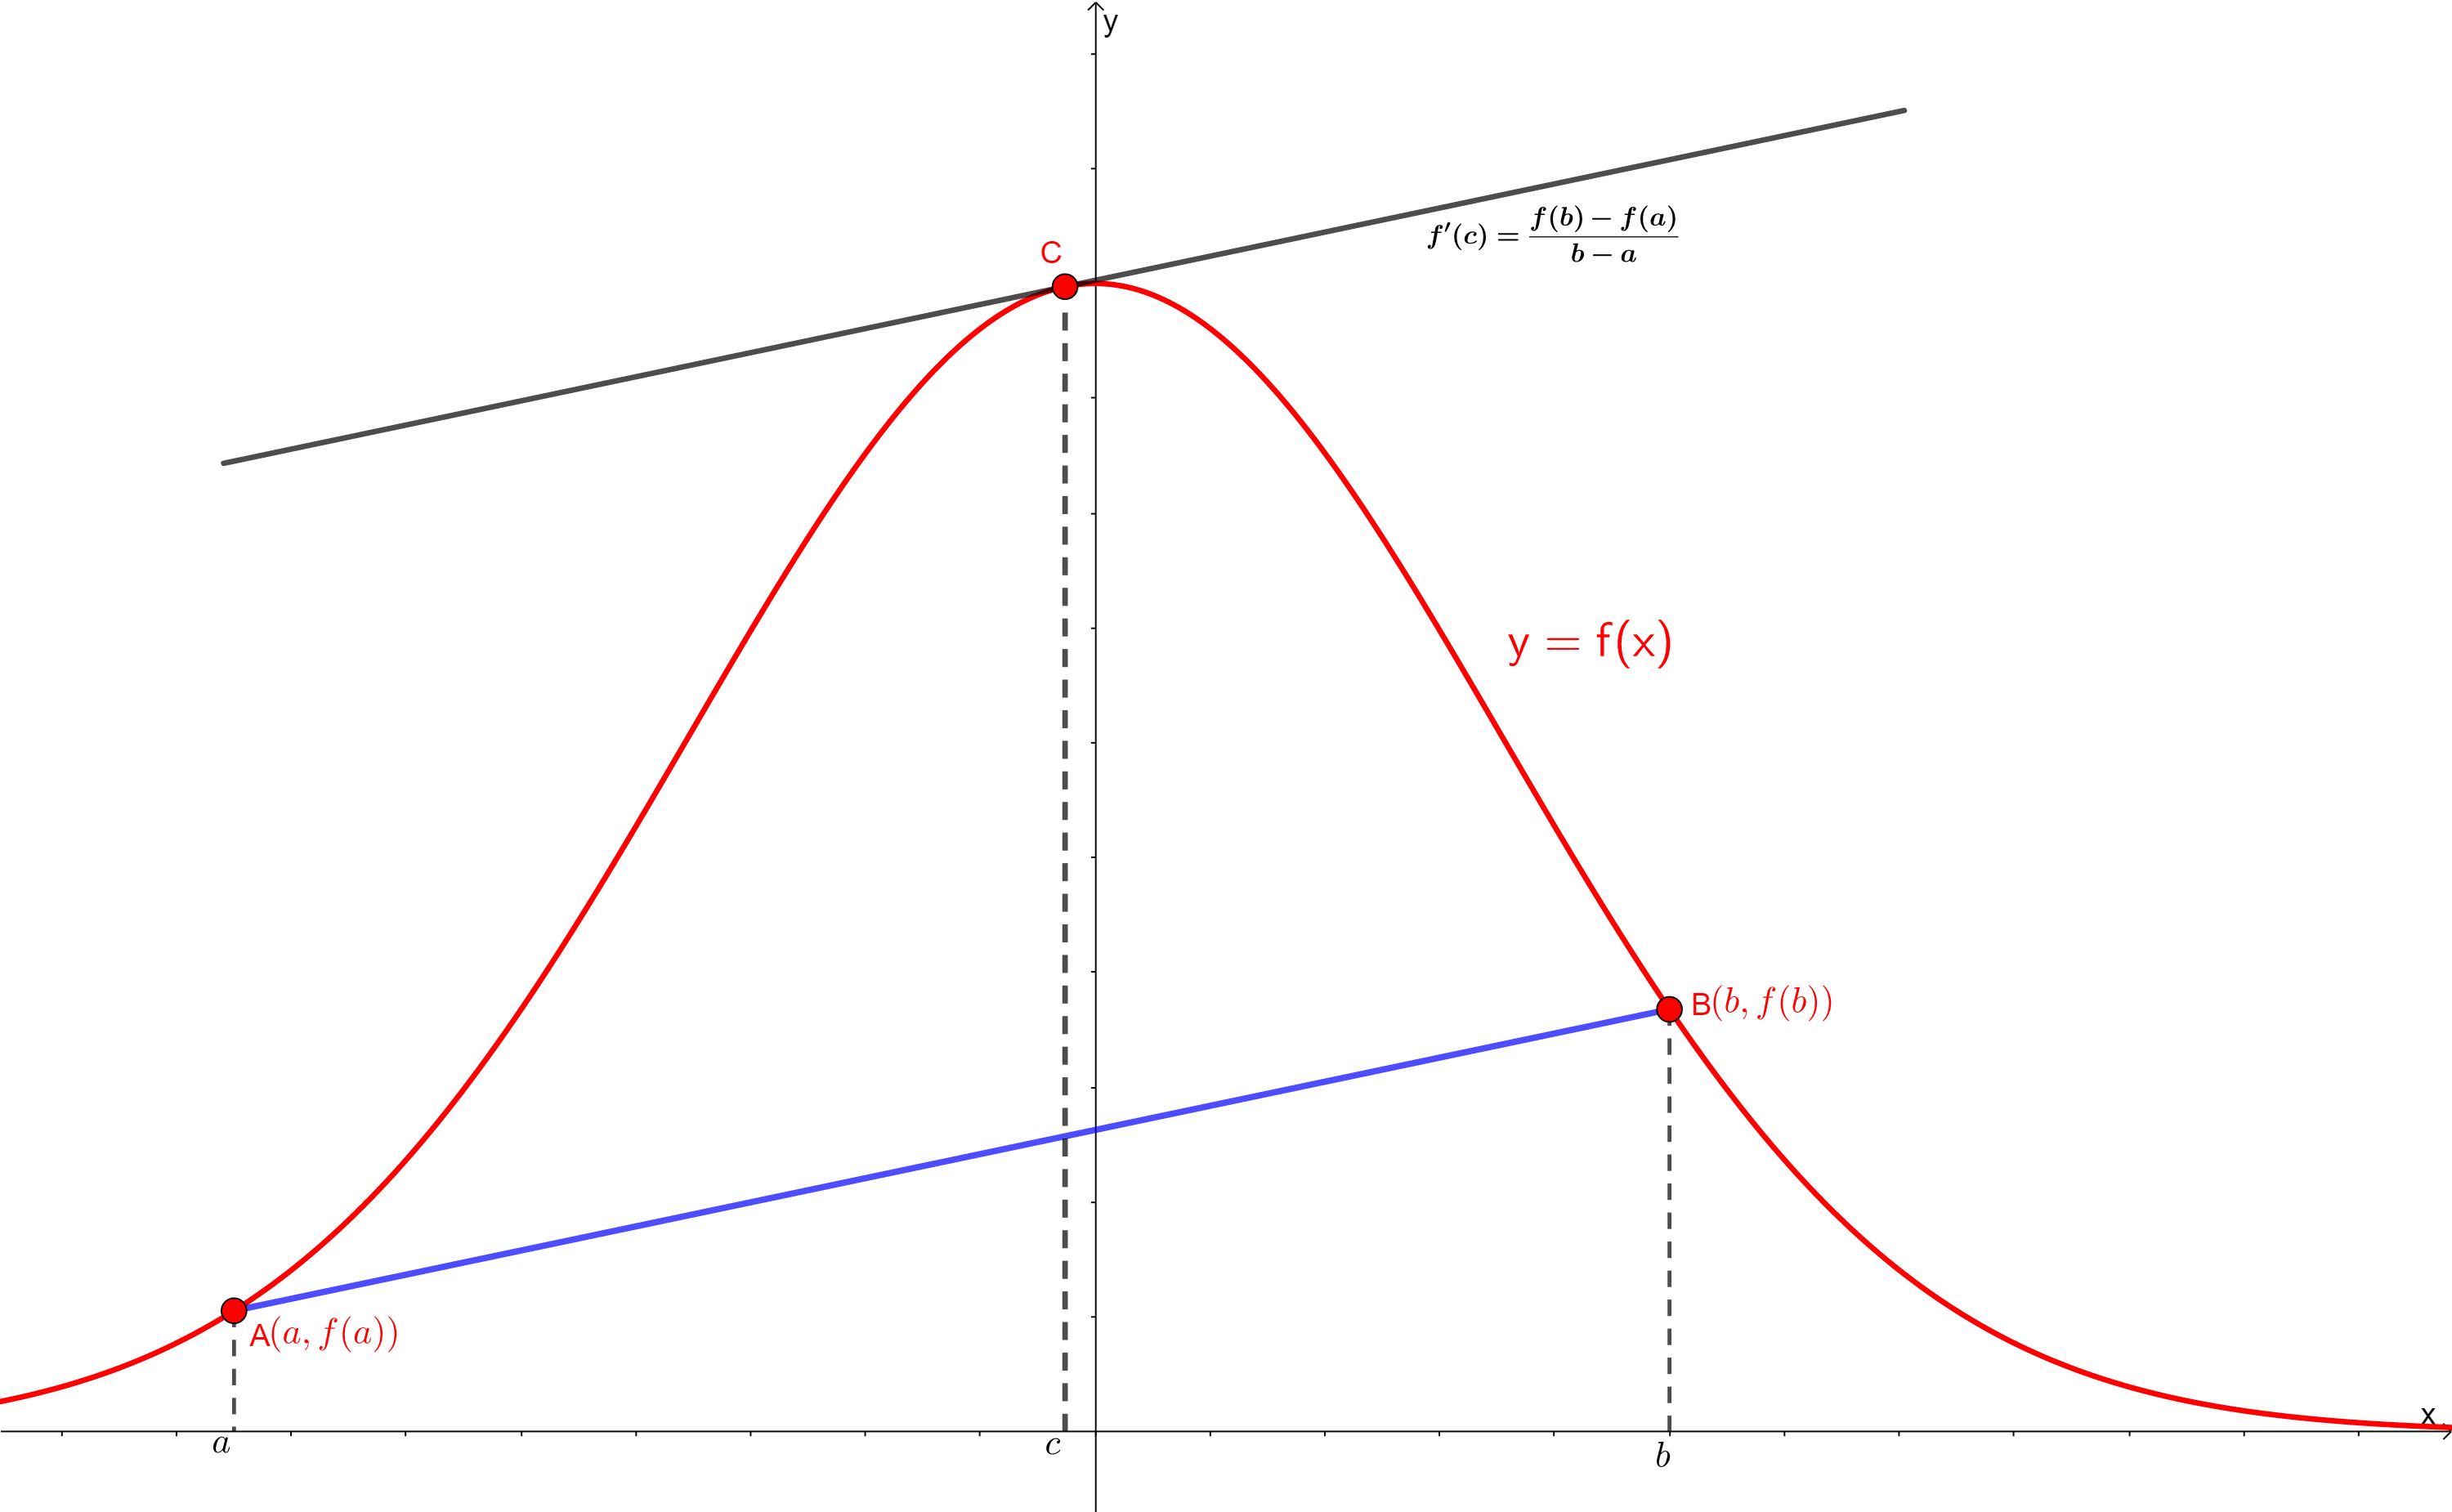
\includegraphics[scale=3.4]{MVT.png}
\subsection{l'Hôpital's Rule}
With l'Hôpital's Rule, limits of $\displaystyle{\frac{0}{0}}$ and $\displaystyle{\frac{\infty}{\infty}}$ indeterminate forms that can only be solved if factorization is made, are solved using differentiation. If the limit is one of the said indeterminate forms $$\lim \limits_{x \to a} \frac{f(x)}{g(x)}=\lim \limits_{x \to a} \frac{f'(x)}{g'(x)} \  .$$
In fact, it appears that any indeterminate forms could be converted to $\displaystyle{\frac{0}{0}}$ or $\displaystyle{\frac{\infty}{\infty}}$ indeterminate forms which can also easily converted to one another. The most used example of this conversion is when the indeterminate expression contains exponential elements, in such a case we can take the whole expression inside a corresponding logarithm since logarithms are continuous functions, and take the exponential part out such that we have changed an exponential indeterminate to $\displaystyle{\frac{0}{0}}$ or $\displaystyle{\frac{\infty}{\infty}}$.
\subsection{Sketching Graphs}
Sketching graphs in a formal way consists of 5 steps:
\begin{enumerate}
\item Find the \textbf{domain} of the function.
\item Find the \textbf{intersections with x and y axis} and possibly some special or easy-to-calculate points that the function is on.
\item Find the \textbf{asymptotes} by checking the \textbf{vertical}, \textbf{horizontal} and \textbf{slant (oblique)} asymptotes. To check the vertical asymptotes one must approach both sides of an undefined point or approach from one side to an end of an undefined interval and see if the limits go to $\pm \infty$ and to check the horizontal asymptotes one must check as x goes to $\pm \infty $ and see if limit converges to a real number. In order to find slant(oblique) asymptotes, long division is made and it is observed if a linear convergence occurs as $x \to \pm\infty$.
\item Apply the \textbf{first derivative test}: By looking at the first derivative, we can find where a functions extrema are, therefore we can know where a function decreases and where it increases. 
\item Apply the \textbf{second derivative test}: Second derivative test is also called the concavity test since it reveals where the function shows upper concavity and where it shows lower concavity. Specifically, the points where $f''(x)=0$ are called the inflection points pointing to the fact that the concavity property changes at that point.
\end{enumerate}
At the end we will have a \textbf{table} that has $f,f'$ and $f''$ on the vertical and the special numbers ($-\infty , $roots, extrema, inflection points$,\infty $) on the horizontal. In that table we will have all the information to draw the graph.
\newpage
\section{Integration}
\subsection{Riemann Sums}
Riemann sums are operations of summations which help calculate the area under a curve, that idea is then combined with limits and integration is obtained. We will see that the increments and subintervals are important in various ways to formulate Riemann sums yet in integration, we could get away with only using the function and the integration variable.

Riemann sums are formulated in 3 ways; Left Riemann Sum, Right Riemann Sum and Mid-point Riemann Sum:

$$\int f(x)dx = \lim \limits_{n \to \infty} \sum \limits_{i=1}^{n} f(x_i^*)(x_i-x_{i-1})$$ where \\For Left Riemann Sum $x_i^*=x_{i-1}$\\For Right Riemann Sum $x_i^*=x_{i}$\\For Mid-point Riemann Sum $\displaystyle{x_i^*=\frac{x_i+x_{i-1}}{2}}$
\subsection{Mean-Value Theorem for Integrals}
If $f$ is continuous on $[a,b]$, then there exists a point c in $[a,b]$ such that $$\int \limits_a^b f(x)dx=(b-a)f(c)$$
\newpage
\subsection{The Fundamental Theorem of Calculus}
Consider that the function $f$ is continuous on an interval $I$ containing the point $a$.
\begin{itemize}
\item[$(i)$] Let the function F be defined on I by $$F(x)=\int \limits_a^x f(t)\ dt.$$ Then $F$ is differentiable on $I$, and $F'(x)=f(x)$ there. Thus, $F$ is an antiderivative of $f$ on $I$.
\item[$(ii)$] If $G(x)$ is any antiderivative of $f(x)$ on $I$, so that $G'(x) = f(x)$ on $I$, then for any $b$ in $I$, we have $$\int \limits_a^b f(x)\ dx=G(b)-G(a)$$
\end{itemize}
\subsection{Techniques of Integration}
\subsubsection{Substitution Method}
$$\int f'(g(x))\ g'(x)\ dx=f(g(x))+C$$ hence defining $u=g(x) \Rightarrow du=g'(x)\ dx$ $$\int f'(u)\ du=f(u) +C$$ proves to be a common way to solve many integrals.
\subsubsection{Inverse Trigonometric Substitutions}
\begin{enumerate}
\item \textbf{arcsin substitution} is applied where integrand consists of $\sqrt{a^2-x^2}$ such that $x= a \cdot \sin (\theta)$ or $\theta = \arcsin (\frac{x}{a})$ hence $\frac{dx}{d\theta}=a\cdot \cos (\theta)$ and since we defined angle $\theta$, we know its all trigonometric values.\\
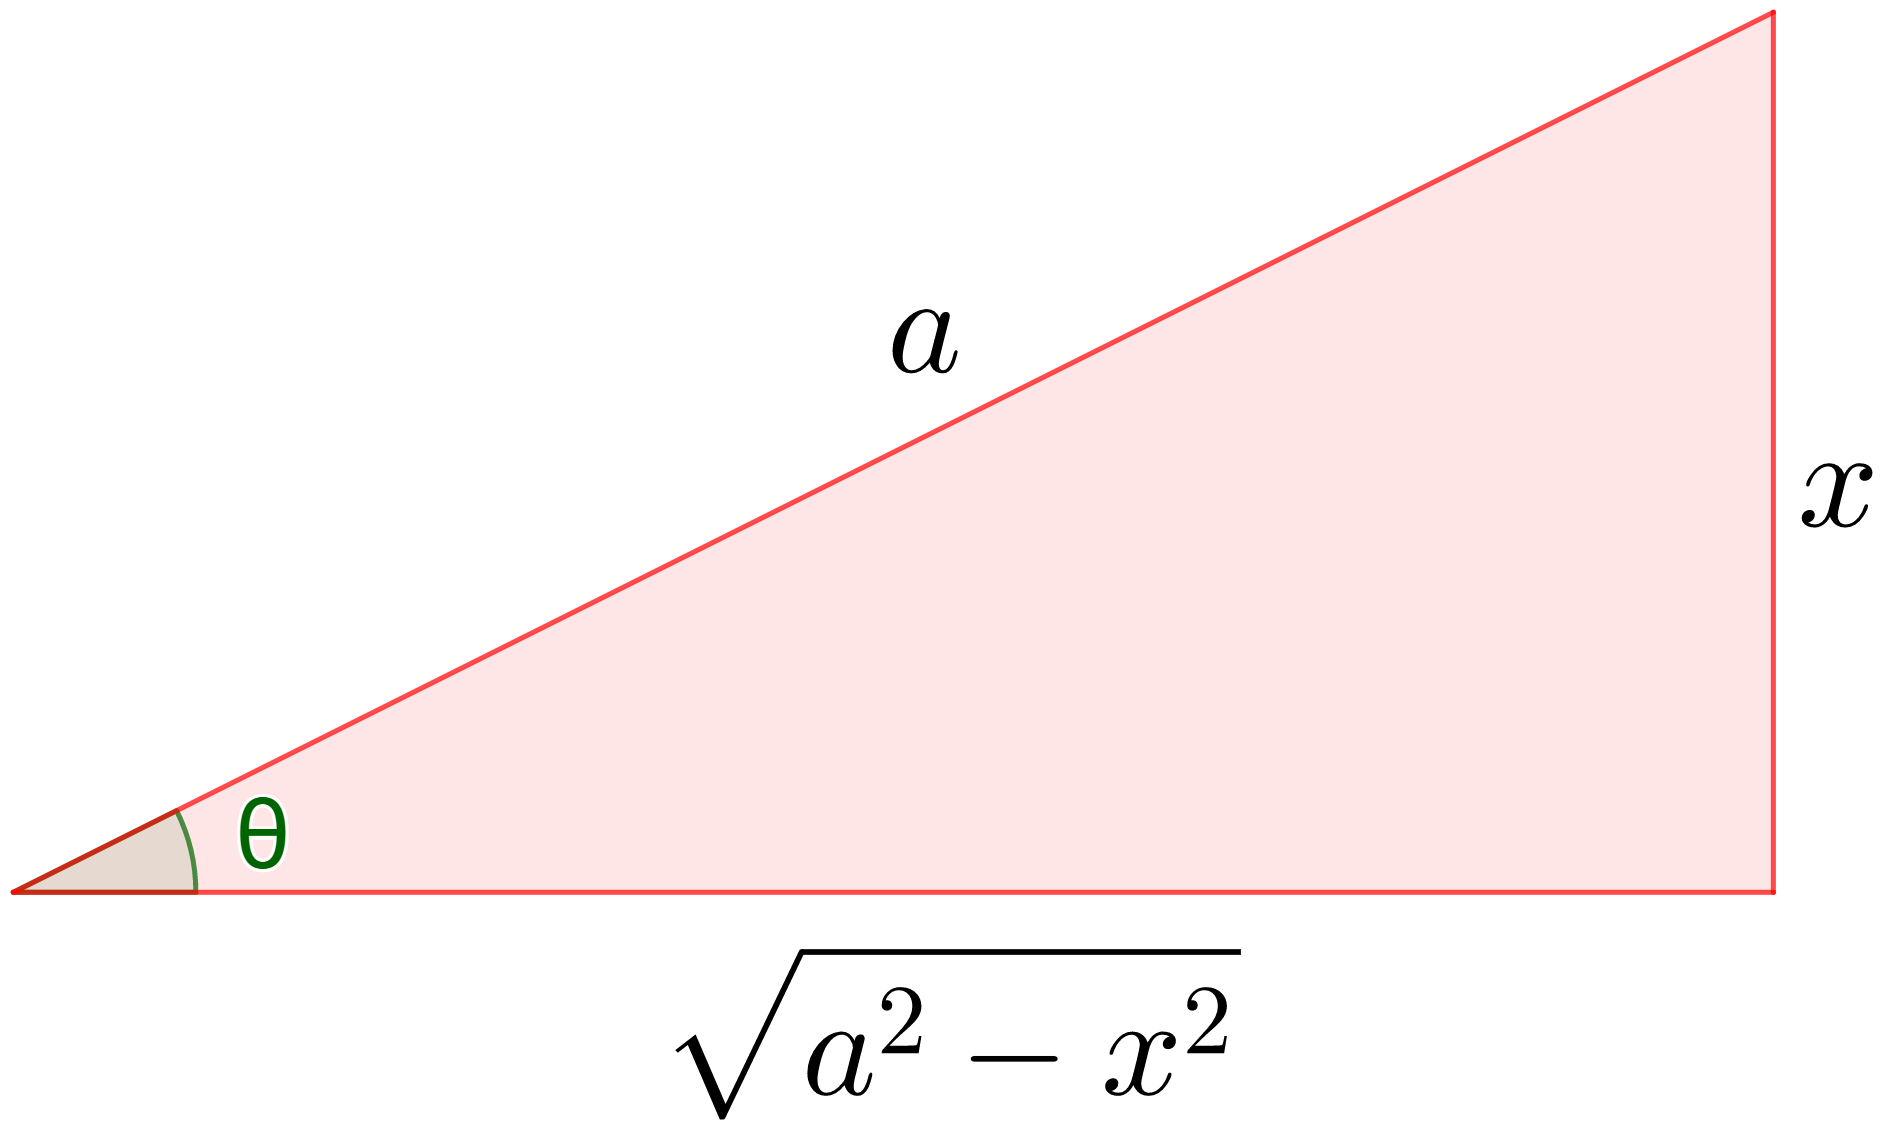
\includegraphics[scale=0.15]{asin_subs.png}
\item \textbf{arctan substitution} is applied where integrand consists of $\sqrt{a^2+x^2}$ such that $x= a \cdot \tan (\theta)$ or $\theta = \arctan (\frac{x}{a})$ hence $\frac{dx}{d\theta}=a\cdot \sec ^2(\theta)$ and since we defined angle $\theta$, we know its all trigonometric values.\\
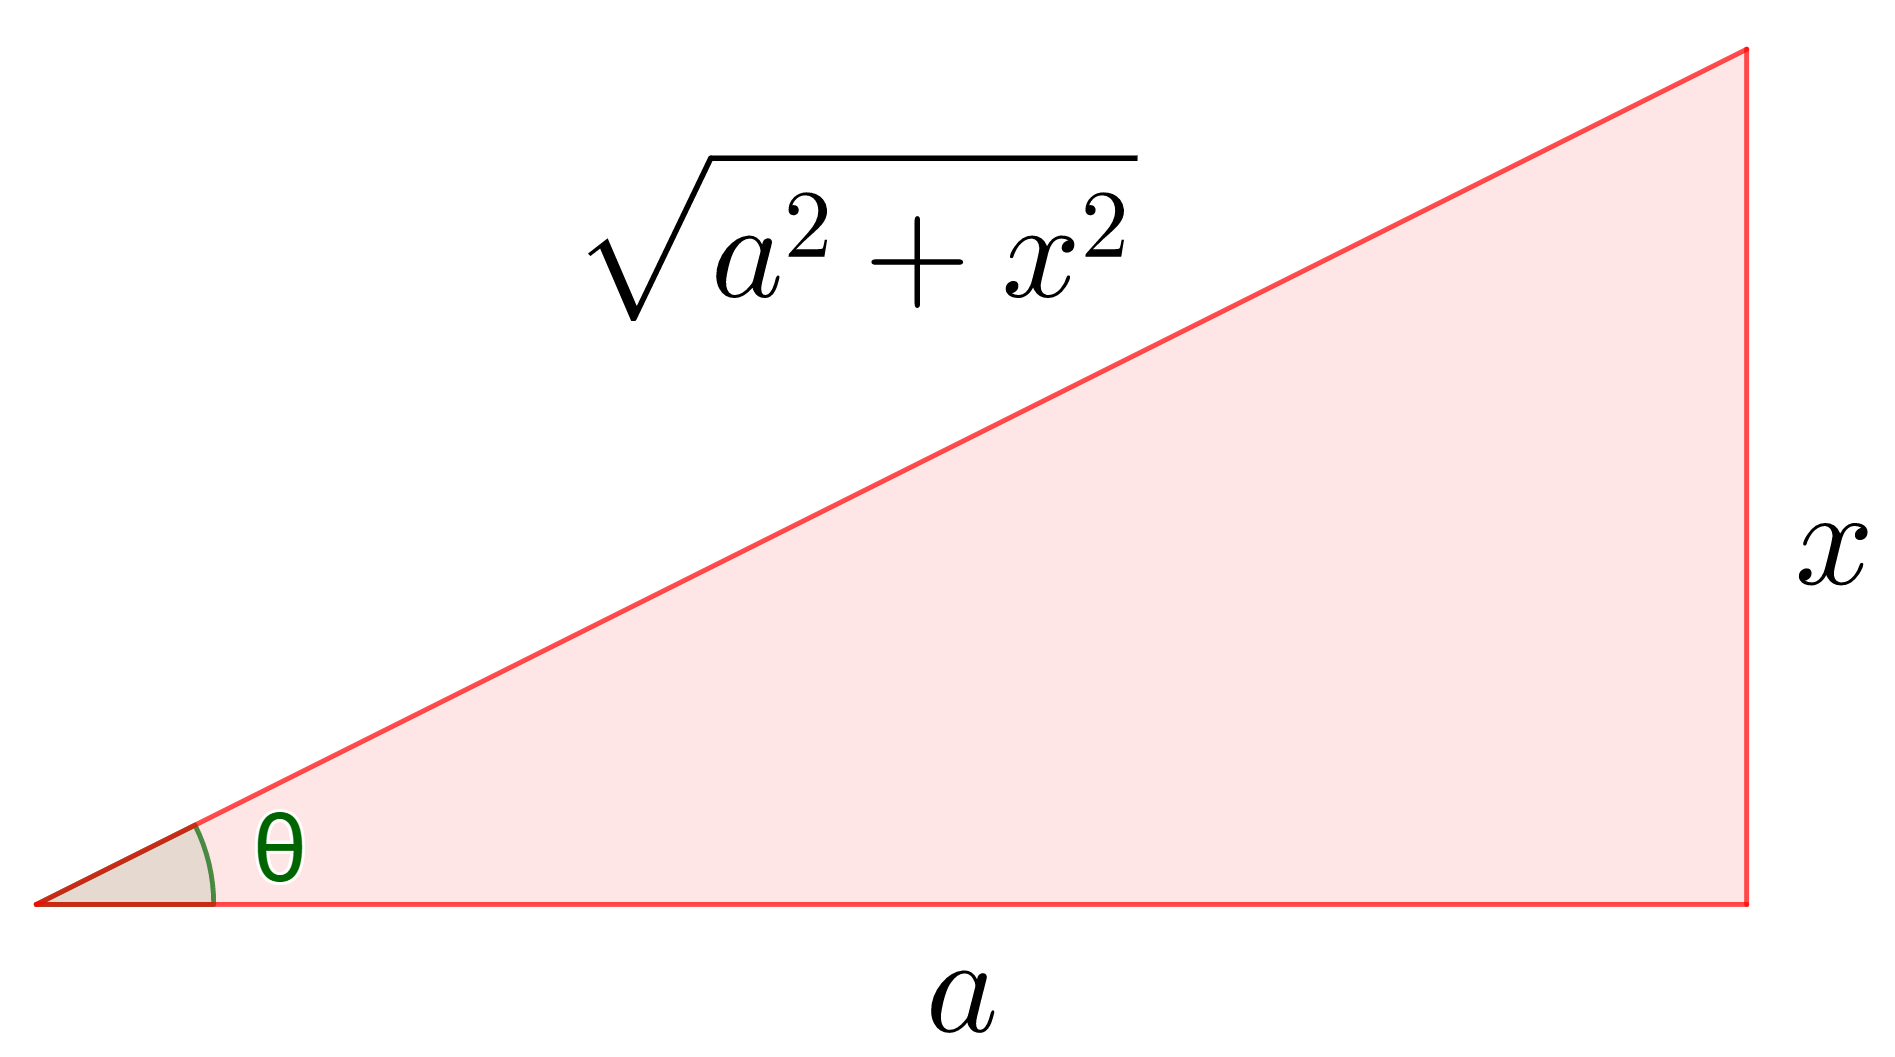
\includegraphics[scale=0.15]{atan_subs.png}
\item \textbf{arcsec substitution} is applied where integrand consists of $\sqrt{x^2-a^2}$ such that $x= a \cdot \sec (\theta)$ or $\theta = \sec ^{-1} (\frac{x}{a})$ hence $\frac{dx}{d\theta}=a\cdot \sec (\theta)\cdot \tan (\theta)$ and since we defined angle $\theta$, we know its all trigonometric values.\\
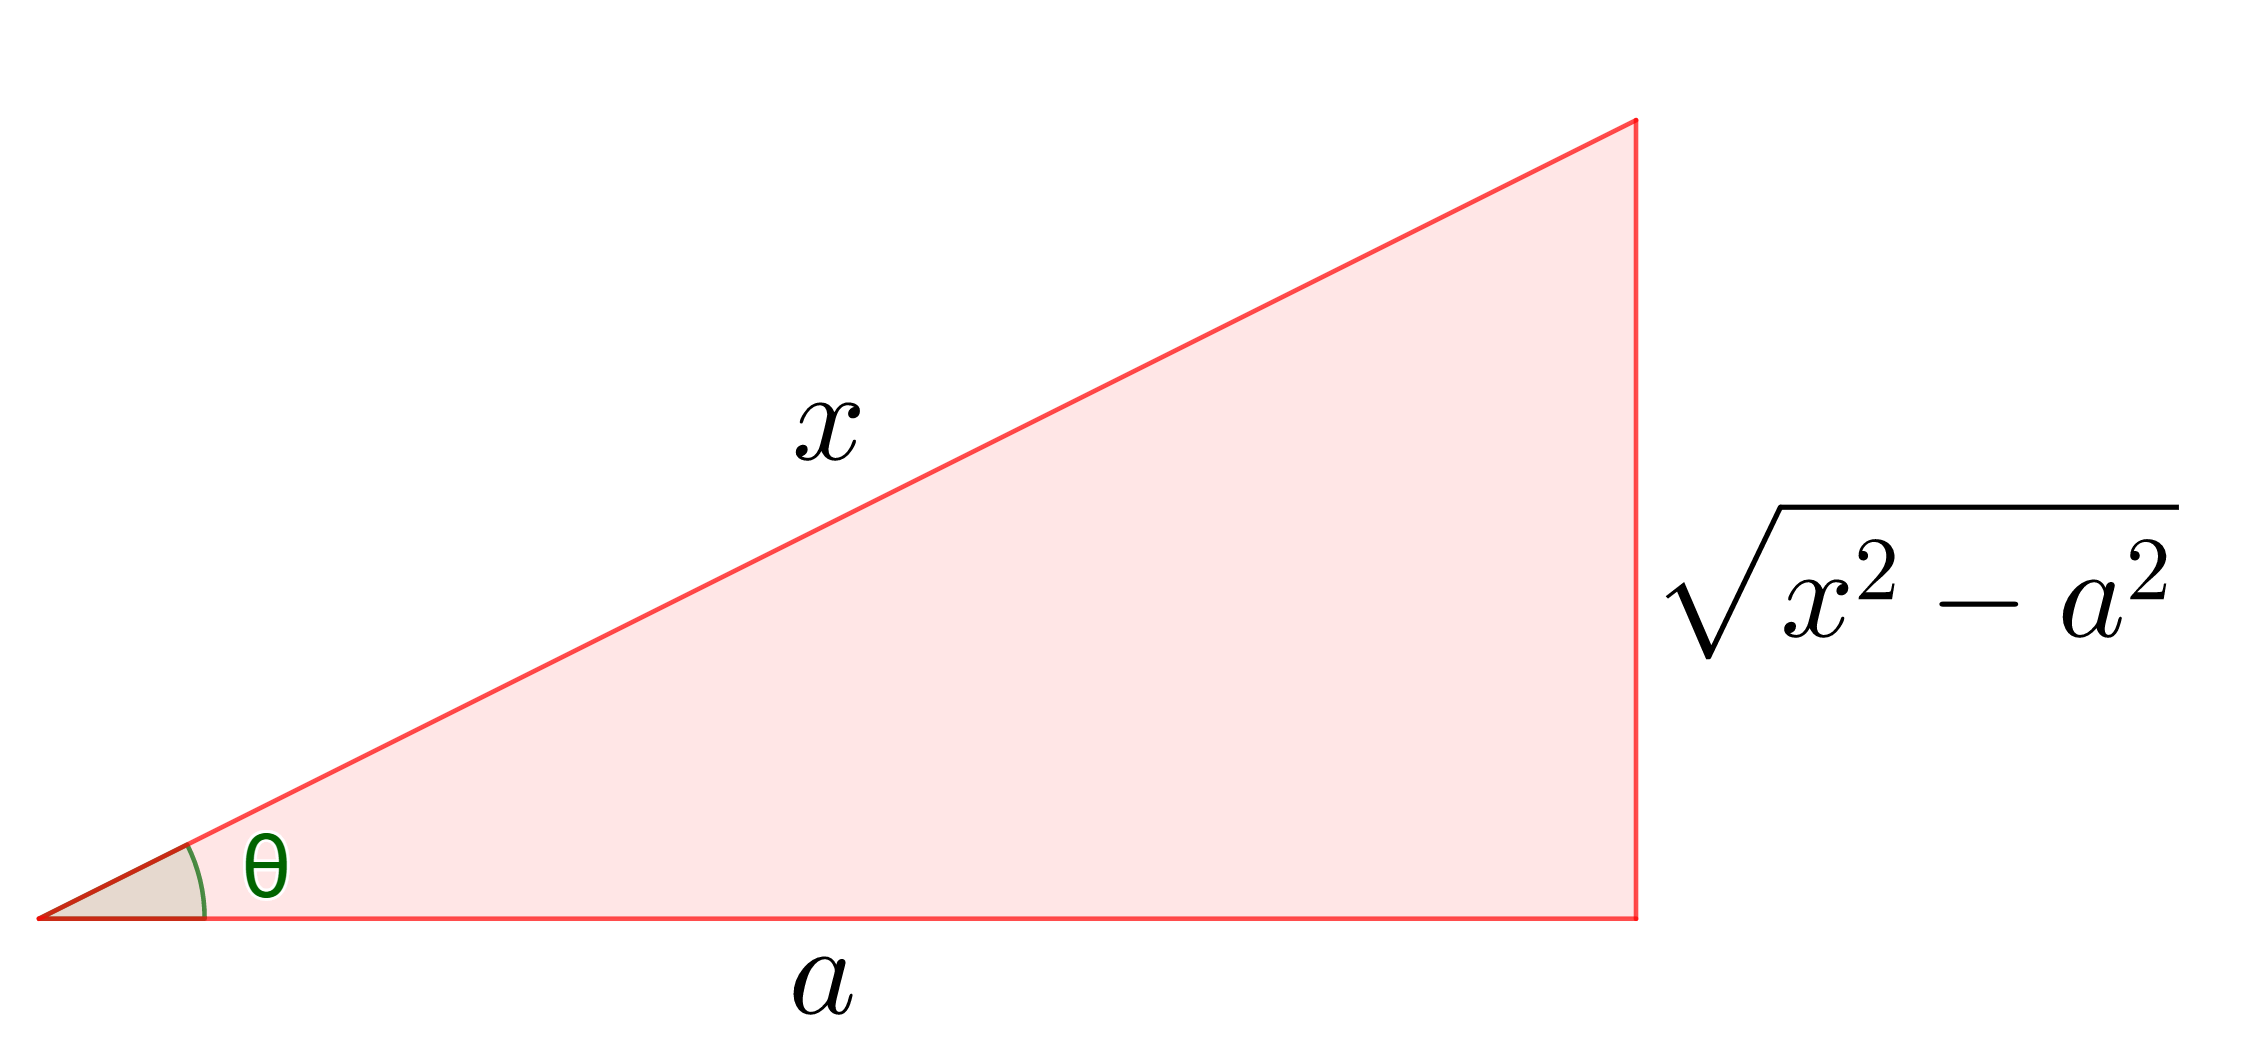
\includegraphics[scale=0.15]{asec_subs.png}
\end{enumerate}
\subsubsection{Weierstrass / Tangent Half-angle Substitution}
In this special substitution, we say $$x = \tan \left(\frac{\theta}{2}\right) \Rightarrow \cos (\theta )=\frac{1-x^2}{1+x^2} ,\ \  \sin (\theta ) = \frac{2x}{1+x^2} , \ \ d\theta = \frac{2dx}{1+x^2}\ \cdots$$ \\ \textbf{Note:}This method is used when there are integrands similar to $\dfrac{1}{a\sin x+b\cos x+c}$
\newpage
\subsubsection{Integration by Parts}
$$\int U(x) dV= U(x)V(x) - \int V(x) dU$$
To select $U$ and $dV$, we have some priorities and rules. Obviously, we need $V(x)$ so $dV$ must be integrable, and for selecting U(x), we have a list of priorities that goes logarithmic, inverse trigonometric, polynomial, trigonometric, exponential from high to low priority. It should be noted that in some integrals a repeating pattern will appear and those loops are not necessarily solvable and the ones that are soluble are made into reduction formulas as a general expression.
\subsubsection{Reduction Formulas}
Reduction formulas appear when the integration by parts fall into a solvable loop.
$$\int \frac{dx}{cos^n x}\,=\, \frac{sin\,x}{\left ( n-1 \right )cos^{n-1}x}\,+\,\frac{\left ( n-2 \right )}{\left ( n-1 \right )}\int \frac{dx}{cos^{n-2}x},\,n\neq1$$ is a famous example.
\subsubsection{Completing Square}
Completing squares in the integrand may yield to expressions which can substituted normally or with inverse trigonometric functions.
\subsubsection{Partial Fractions Method}
When dealing with integrals like $\displaystyle{\int \frac{P(x)}{Q(x)}}$ where $P(x)$ and $Q(x)$ are polynomials and degree of P is smaller than Q, we factorize the denominator first. For linear factors in form $(x-r)^m$ we write $\displaystyle{\frac{A}{x-r} +\frac{B}{(x-r)^2} \cdots}$ and for quadratic factors in form $(ax^2+bx+c)^n$ we write $\displaystyle{\frac{Ax+B}{ax^2+bx+c} +\frac{Cx+D}{(ax^2+bx+c)^2} \cdots}$ and so on, solve the system for the unknowns, which can be quite cumbersome, then solve the integral. 
\newpage
\subsection{Improper Integrals}
Improper integrals are when the integrals have on at least one of their boundaries, $\infty $ or $-\infty $ or there is a \textbf{discontinuous point} of the integrand function in between the integral boundaries. In case of an infinity on the integral boundaries, we replace the infinity with a placeholder variable and take the limit on infinity, take the integral conserving placeholder variable and at the last step, taking the limit. In case of a discontinuous point between integral boundaries, we divide the integral to parts from the discontinuous point(s) and again, replacing the discontinuous point(s) on the integral boundary with a placeholder variable and taking the limit. If in the end of the operation the limit yields a real number, we call such improper integrals "convergent" and If not, "divergent".
\subsection{Some Important Elementary Integrals}
$$\int \ln (x)dx=x\cdot \ln (x)-x+C$$
$$\int \frac{1}{x}dx=\ln |x| +C$$
$$\int \sec (x)dx=\ln \left|\sec (x)+\tan (x)\right| +C$$
$$\int \tan x\ dx=\ln |\sec x| +C$$
\newpage
\subsection{Volumes by Slicing}
$$V=\int \limits_a^b A(x)\,dx$$
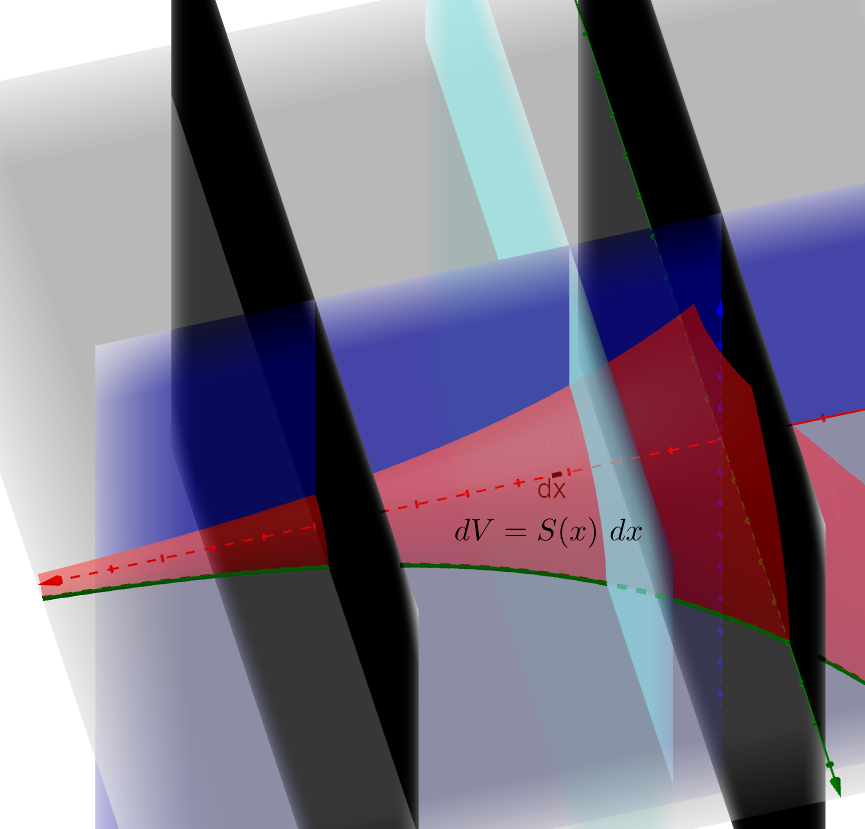
\includegraphics[scale=0.6]{Slicedvol.png}
\newpage
\subsection{Solids of Revolution}
\subsubsection{Disk Method}

\begin{figure}[H]
\centering
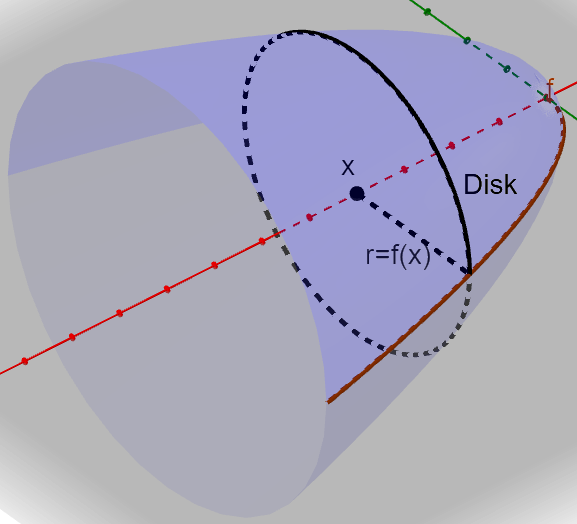
\includegraphics[scale=0.7]{disk.png}
\caption{In this method, an infinitesimal volume part is considered to be a cylinder with base radius of $f(x)$ and the thickness of $dx$.}
\end{figure}

Rotation about x axis: $$V=\pi \int \limits_a^b f^2(x)\,dx$$
Rotation about y axis: $$V=\pi \int \limits_c^d f^2(y)\,dy =\pi \int \limits_a^b x^2\,f'(x)\,dx $$
Rotation about $y=-c$ : $$V=\pi \int \limits_a^b (f(x)+c)^2\,dx$$
\newpage
\subsubsection{Washer Method}
Rotation about $y=-c$ : $$V=\pi \int \limits_a^b (f(x)+c)^2-(g(x)+c)^2\,dx\ .$$ The same passes for rotations about vertical lines, only the functions will be made of variable y.
\begin{figure}[H]
\centering
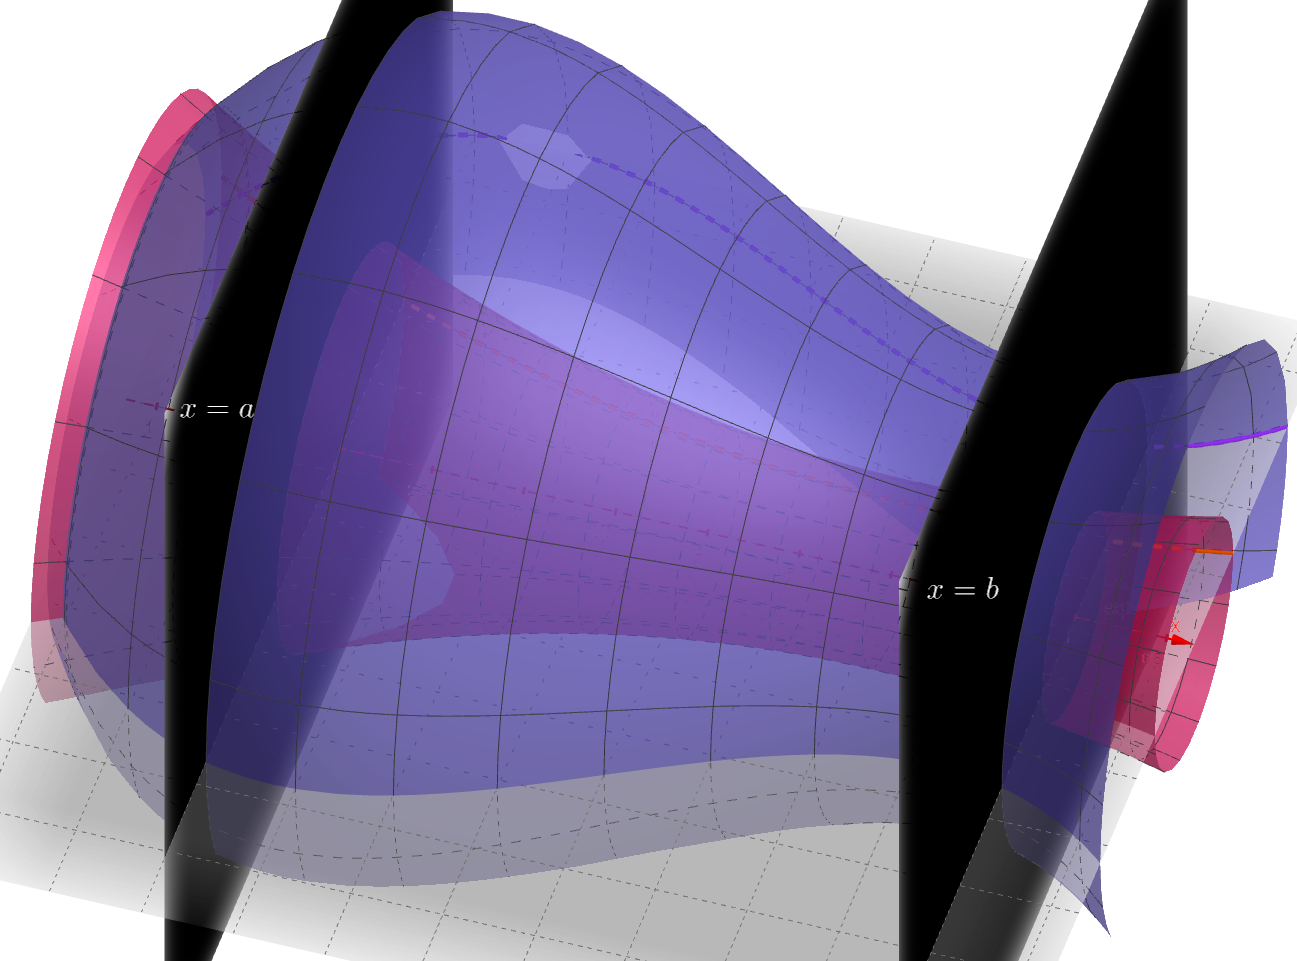
\includegraphics[scale=0.42]{washer.png}
\caption{The washer method includes two disks that are subtracted from each other.}
\end{figure}
\newpage
\subsubsection{Cylindrical Shells Method}
The shell method is about considering the cylindrical shell constructed by the rotation of an infinitesimal area, the cylindrical shell volume $dV=2\pi r\,dS$, note that both $r$ and $S$ are functions of x (or y depending on respective axis).


Shell radius at x axis (rotation about y axis): $$V=2\,\pi \int \limits_a^b x\,f(x)\,dx $$ the variables replaced by y is the integral of shell radius at y axis (rotation about x axis). It must be noted that the cylindrical shell method and disk/washer methods have the opposite integral variables for any axis rotation, in this sense we expect that for any solid of revolution, one of these methods will yield easier solution.\\
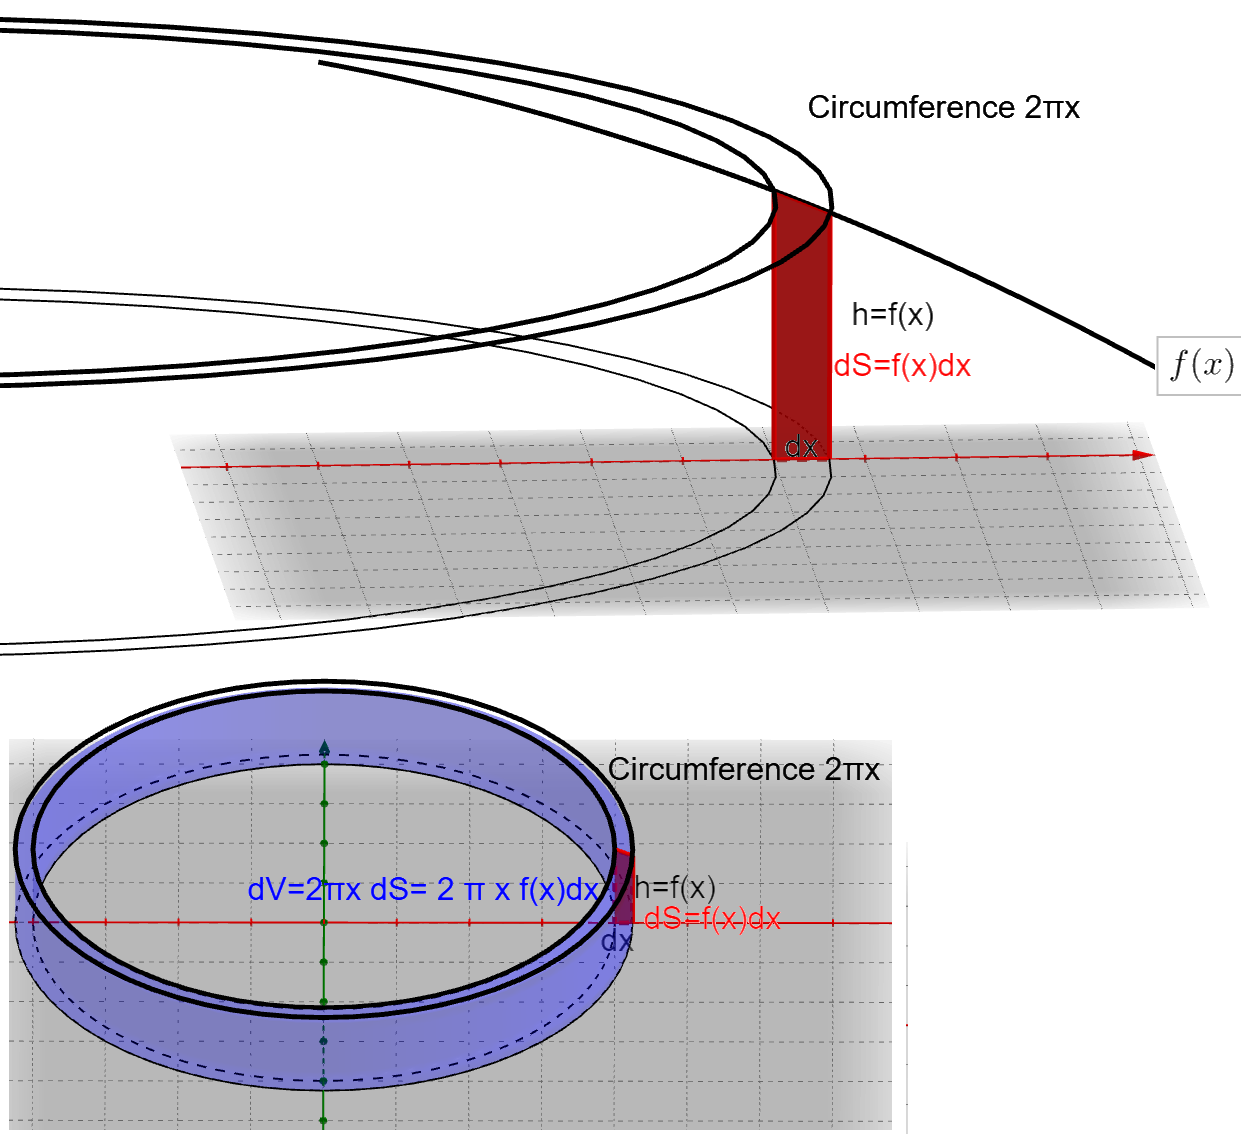
\includegraphics[scale=0.446]{shell.png}
\newpage
\subsection{Arc Length}
Since $dL=\sqrt{dx^2+dy^2}$ and $dy=f'(x)\,dx$ $$dL=|dx|\sqrt{1+(f'(x))^2} \Rightarrow L=\int \limits_a^b \sqrt{1+(f'(x))^2} \,dx$$
\subsection{Surface Area}
Area of a surface of revolved around x axis- integral with respect to x: $$A=2\pi \int \limits_a^b |f(x)|\sqrt{1+(f'(x))^2} \,dx$$
Area of a surface of revolved around x axis- integral with respect to y: $$A=2\pi \int \limits_c^d |y|\sqrt{1+(g'(y))^2} \,dy$$
Area of a surface of revolved around y axis- integral with respect to x: $$A=2\pi \int \limits_a^b |x|\sqrt{1+(f'(x))^2} \,dx$$
Area of a surface of revolved around y axis- integral with respect to y: $$A=2\pi \int \limits_c^d |g(y)|\sqrt{1+(g'(y))^2} \,dy$$
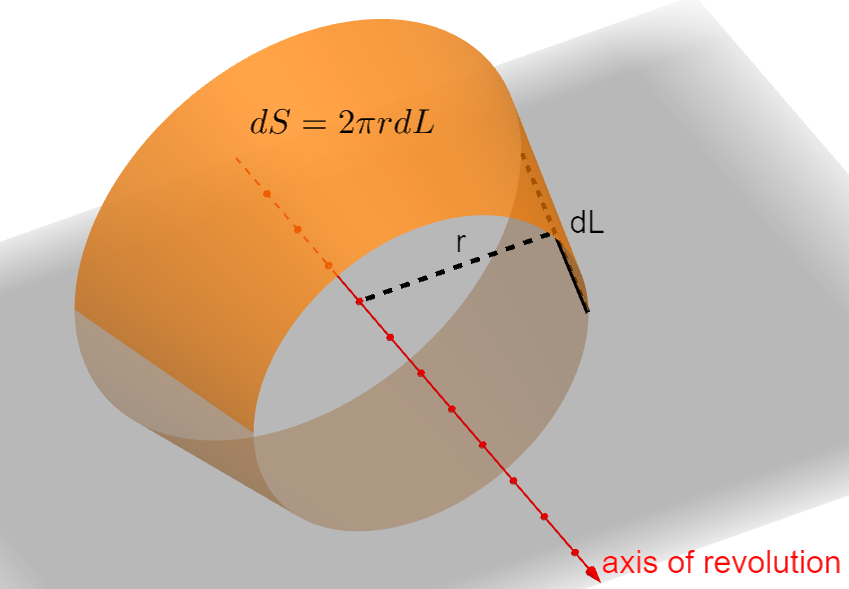
\includegraphics[scale=0.40]{surfacearea.png}
\section{Sequences and Series}
\subsection{Defining Sequences and Series}
Sequences are functions that are defined to take inputs in natural numbers.\\
Series are summations of elements of a sequence.
\subsection{Properties of Sequences}
Since sequences are actually functions, the general operations on sequences are very similar to the functions that are defined on the real numbers set. We have the same limit properties, the squeeze theorem for sequences. It must be noted that most sequences have corresponding functions that are defined on the real numbers (even factorials can be functionalized ($\Gamma$ function) or approximated (Stirling's Approximation) to a function of real numbers) and as such the sequence's limit when $n \to \infty =$ function's limit when $x \to \infty$.
\subsubsection{Terms for describing Sequences}
\textbf{Bounded Sequences}: The sequence $a_n$ is bounded below by L if $a_n\geq L\ ,\forall n\in \mathbb{N} ^+$ and bounded above by M if $a_n\leq M\ ,\forall n\in \mathbb{N} ^+$. If a sequence is both bounded below and bounded above, then it is called to be bounded. If a sequence is below bounded by 0, then it is a positive sequence and if a sequence is above bounded by 0, then it is a negative sequence. 

\textbf{Increasing/Decreasing Sequences}: The sequence $a_n$ is increasing if \\ $a_{n+1}\geq a_n\ , \forall n\in \mathbb{N} ^+$ and it is decreasing if $a_{n+1}\leq a_n\ , \forall n\in \mathbb{N} ^+$. A sequence is said to be monotonic if it is either increasing or decreasing.

\textbf{Alternating Sequences}: The sequence $a_n$ is said to be alternating if \\ $a_n\cdot a_{n+1}<0\ , \forall n\in \mathbb{N} ^+$

If a sequence appears to show one of these properties when $n\geq c$ where $c>1$, the sequence is said to show the property ultimately.
\subsubsection{Bounded Monotonic Convergence Theorem}
The theorem states that \textbf{a monotonic sequence is convergent if it's bounded}. Specifically, an \textbf{increasing} sequence is \textbf{convergent} if it is \textbf{bounded above} and a \textbf{decreasing} sequence is \textbf{convergent} if it is \textbf{bounded below}. Also, a \textbf{convergent sequence is bounded}.
\subsection{Special Series}
\subsubsection{Geometric Series}
A series of form $\displaystyle{\sum \limits_{n=1}^\infty a\cdot r^{n-1}}$. The number a is the first term and r is called the common ratio. $\displaystyle{s_n=\frac{a(1-r^n)}{1-r}}$. A geometric series converge if $a=0$ or $|r|<1$ and converges to $\displaystyle{\frac{a}{1-r}}$
\subsubsection{Telescoping Series}
Telescoping series are series whose partial sums \textbf{fold up into a simple form when the terms are expanded}. The method of partial fractions are also useful to use with telescoping series. One famous telescoping series is: $$\sum \limits_{n=1}^\infty \frac{1}{n(n+1)} = 1\ .$$
\newpage
\subsection{Using Integrals to Estimate the Sum of a Series}
$$\int \limits_{n+1}^\infty f(x)\,dx\leq \sum \limits_{x = n+1}^\infty f(x)\leq \int \limits_{n}^\infty f(x)\,dx$$ where $f(x)$ is a positive, continuous and nonincreasing function.\\
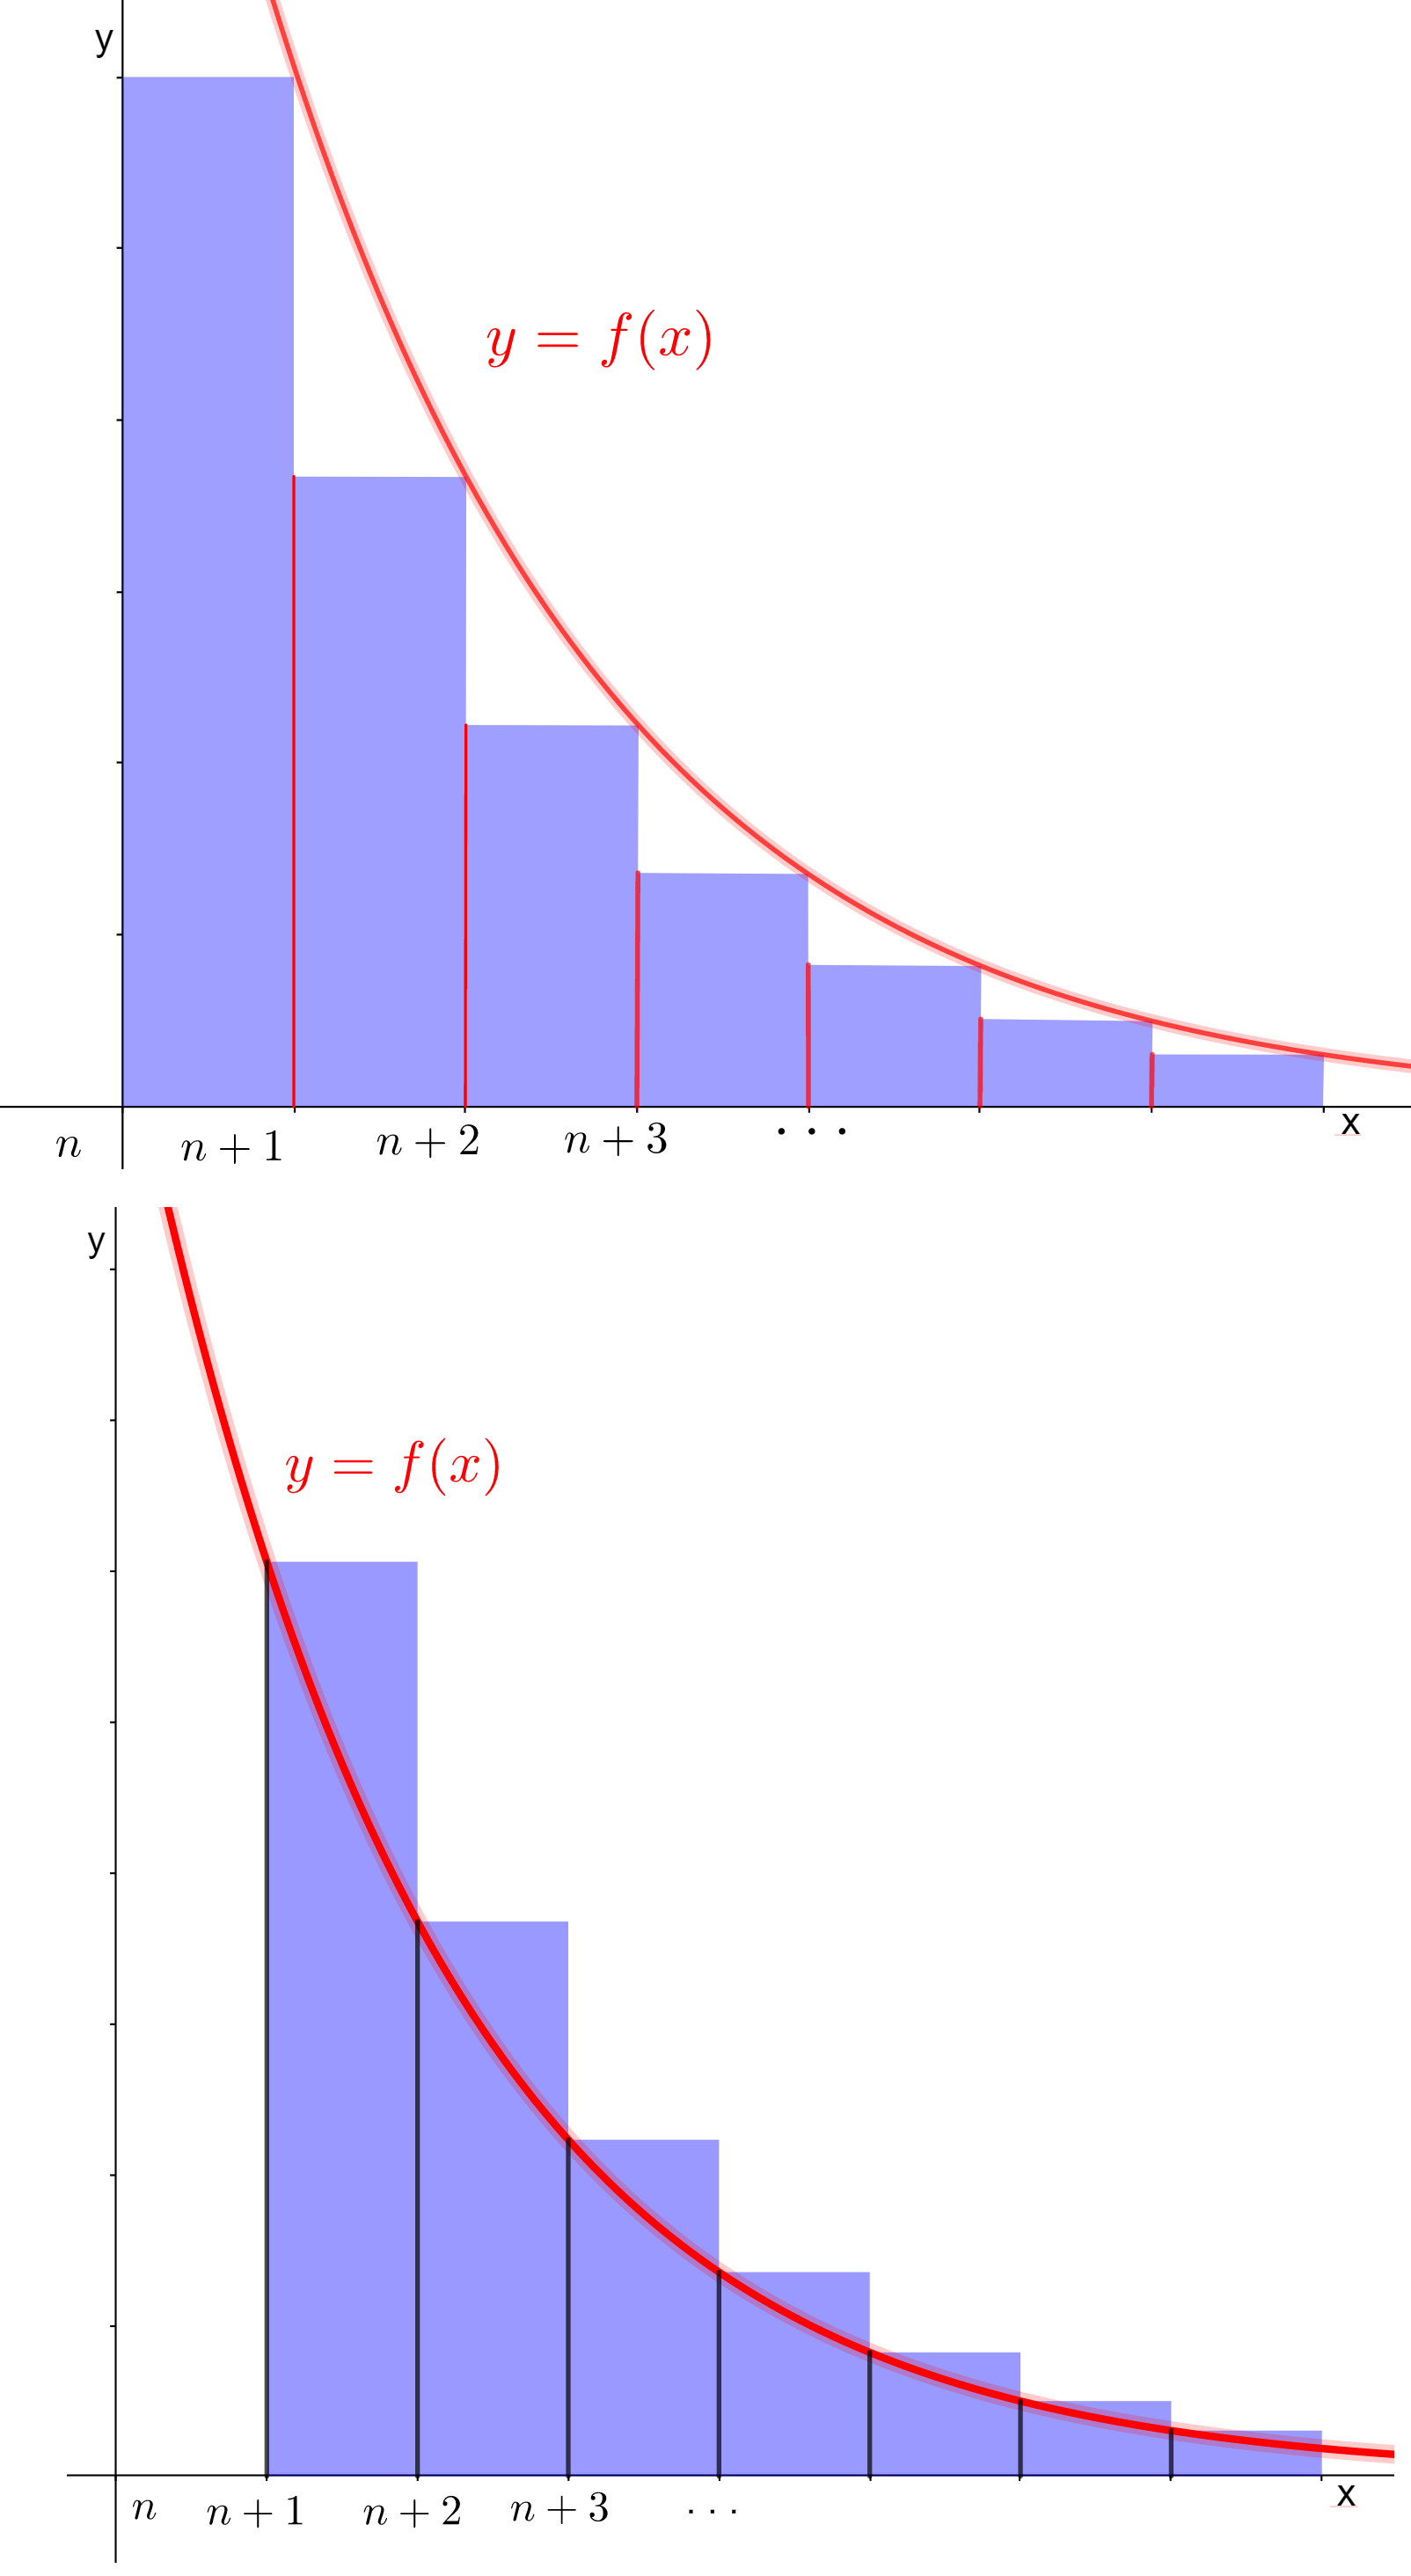
\includegraphics[scale=0.23]{seriesintegral.png}
\newpage
\subsection{Convergence Tests and Conditions for Series}
\begin{small}
\begin{enumerate}
\item $\displaystyle{\sum \limits_{n=1}^\infty a_n}$ converges if and only if $\displaystyle{\sum \limits_{n=N}^\infty a_n}$ where $N\geq 1$.
\item \textbf{Geometric Series Test}: If $|r|<1$ then $\displaystyle{\sum \limits_{n=0}^\infty a r^n = \frac{a}{1-r}}$.
\item \textbf{Divergence Test}: If $\sum a_k$ \textbf{converges}, then $\lim \limits_{k \to \infty} a_k=0$. In other words, If $\lim \limits_{k \to \infty} a_k\neq 0$ then $\sum a_k$ \textbf{diverges}.

\item \textbf{Integral Test}: Suppose that $a_n = f(n)$, where $f$ is \textbf{positive, continuous and nonincreasing} on interval $[N,\infty)$ for some positive integer N. Then $\sum \limits_{n=1}^\infty a_n$ and $\int \limits_N^\infty f(t)\,dt$ either \textbf{both converge or both diverge}.
\item \textbf{The P-series Test}: $\displaystyle{\sum \frac{1}{n^p}}$ where $p\in \mathbb{R}$ \textbf{converges} if $p>1$ and \textbf{diverges} if $p\leq 1$.
\item \textbf{The Comparison Test}: Let $0\leq a_k \leq b_k$ at least ultimately. If $\sum b_k$ is \textbf{convergent} then $\sum a_k$ is \textbf{convergent} and if $\sum a_k$ is \textbf{divergent} then $\sum b_k$ is \textbf{divergent}.
\item \textbf{The Limit Comparison Test}: If $a_k>0$ , $ b_k>0$ and $\displaystyle{\lim \limits_{k \to \infty} \frac{a_k}{b_k}=L}$ where $L\in \mathbb{R} ^+$, $\sum a_k$ and $\sum b_k $ \textbf{both converge or both diverge}.
\item \textbf{The $0 - \infty$ Limit Comparison Test}: Assuming $a_k>0$ and $b_k>0$:
\begin{enumerate}
\item If $\lim \limits_{k \to \infty} \frac{a_k}{b_k}=0$ and $\sum b_k$ \textbf{converges}, then $\sum a_k$ also \textbf{converges}.
\item If $\lim \limits_{k \to \infty} \frac{a_k}{b_k}=\infty$ and $\sum b_k$ \textbf{diverges}, then $\sum a_k$ also \textbf{diverges}.
\end{enumerate}
\item \textbf{The Ratio and Root Tests}: If $a_k>0$ and $\displaystyle{\lim \limits_{k \to \infty} \frac{a_{k+1}}{a_k}=L}$ or $\displaystyle{\lim \limits_{k \to \infty} \sqrt[k]{a_k}=L}$ 
\begin{enumerate}
\item $L<1 \Rightarrow \sum a_k$ \textbf{converges}.
\item $L=1 $, then the test is \textbf{inconclusive}.
\item $L>1 \Rightarrow \sum a_k$ \textbf{diverges}.
\end{enumerate}
\item \textbf{Leibniz's Alternating Series Test}: $\sum (-1)^{k+1} a_k$ where $a_k>0$ \textbf{converges} if $\lim \limits_{k \to \infty} a_k=0$ and $a_k$ is a \textbf{decreasing sequence}.
\item \textbf{Absolute Convergence Test}: If $\sum |a_k|$ \textbf{converges}, then $\sum a_k$ is said to be \textbf{absolute convergent} and if a series is \textbf{absolute convergent} then it is also \textbf{convergent} but the \textbf{inverse is not correct}.
\end{enumerate}
\end{small}
\subsection{Power Series}
A series of form $\displaystyle{\sum \limits_{n=0}^\infty a_n(x-c)^n}$ where $c$ is called to be the \textbf{centre of convergence} and for any power series of said form one of the following must hold:
\begin{enumerate}
\item the series may converge only at x=c,
\item the series may converge at every real number or
\item there may exist a positive real number $R$ such that the series converges at every x satisfying $|x-c|<R$ and diverges at every other x values. In this case the two endpoints which are $x=c+R$ and $x=c-R$ must be checked for convergence individually. \textbf{$R$ here is called the radius of convergence}. 
\end{enumerate}
If $\displaystyle{\lim \limits_{k \to \infty} \left|\frac{a_{k+1}}{a_k}\right|=L}$ or $\displaystyle{\lim \limits_{k \to \infty} \sqrt[k]{|a_k|}=L}$ and if:
\begin{enumerate}
\item $0<L<\infty$: then the power series is convergent where $\displaystyle{|x-c|<R=\frac{1}{L}}$ and the \textbf{endpoints of the interval must be individually checked for convergence}.
\item $L=0$: then the series converges $\forall x\in \mathbb{R}$.
\item $L=\infty$: then the series only converge for $x=c$.
\end{enumerate}
\subsubsection{Operations on Power Series}
\begin{enumerate}
\item Multiplication using \textbf{Cauchy product}: $$\left(\sum \limits_{n=0}^\infty a_nx^n\right) \left(\sum \limits_{n=0}^\infty b_nx^n\right) = \sum \limits_{n=0}^\infty \left( \sum \limits_{j=0}^n a_jb_{n-j}\right) x^n .$$ 
\item \textbf{Differentiation} and \textbf{integration} can be done \textbf{term-by-term} or on the \textbf{general term of the series} since integration and differentiation are continuous operations, it must be noted that the centre and the radius of convergence does not change after differentiation or integration operations however, the openness and closeness of the interval endpoints may change.
\end{enumerate}
\subsection{Taylor and Maclaurin Series}
Taylor series are series of form $$\sum \limits_{n=0}^\infty \frac{f^{(n)}(c)}{n!}\,(x-c)^n.$$
Maclaurin series are Taylor series with centre of convergence at $x=0$.
$${{e^x} = \sum\limits_{n = 0}^\infty  {\frac{{{x^n}}}{{n!}}}  }={ 1 + x + {\frac{{{x^2}}}{{2!}}} }+{ {\frac{{{x^3}}}{{3!}}} +  \ldots} \ \ \ \ \ \ \ \forall x\in \mathbb{R}$$
$${\cos x = \sum \limits_{n = 0}^\infty  {\frac{{{{\left( { - 1} \right)}^n}{x^{2n}}}}{{\left( {2n} \right)!}}} }={ 1 - {\frac{{{x^2}}}{{2!}}} }+{ {\frac{{{x^4}}}{{4!}}} }-{ {\frac{{{x^6}}}{{6!}}} +  \ldots } \ \ \ \ \ \ \ \forall x\in \mathbb{R}$$
$${\sin x = \sum\limits_{n = 0}^\infty  {\frac{{{{\left( { - 1} \right)}^n}{x^{2n + 1}}}}{{\left( {2n + 1} \right)!}}}  }={ x - {\frac{{{x^3}}}{{3!}}} }+{ {\frac{{{x^5}}}{{5!}}} }-{ {\frac{{{x^7}}}{{7!}}} +  \ldots} \ \ \ \ \ \ \ \forall x\in \mathbb{R}$$
$$\frac{1}{1-x}=\sum \limits_{n=0}^\infty x^n=1+x+x^2+x^3+\ldots \ \ \ (-1< x < 1)$$
$$\frac{1}{(1-x)^2} = \sum \limits_{n=1}^\infty nx^{n-1} = 1+2x+3x^2+4x^3+\ldots \ \ \ (-1< x < 1)$$
$$\ln (1+x) = \sum \limits_{n=1}^\infty \frac{(-1)^{n-1}\cdot x^n}{n}=x-\frac{x^2}{2}+\frac{x^3}{3}-\frac{x^4}{4} + \ldots \ \ \ (-1\leq x \leq 1)$$
$$\arctan x=\sum \limits_{n=0}^\infty \frac{(-1)^n}{2n+1}x^{2n+1} = x -\frac{x^3}{3}+\frac{x^5}{5}-\frac{x^7}{7}+\ldots \ \ \ (-1\leq x \leq 1)$$
\subsubsection{Taylor's Theorem}
$f(x)=P_n(x)+E_n(x)$ is Taylor's Formula where $P_n(x)=\sum \limits_{k=0}^n \frac{f^{(k)}(c)}{k!} (x-c)^k$ is the Taylor Polynomial and $E_n(x)=\frac{f^{(n+1)(s)}}{(n+1)!}(x-c)^{n+1}$ for some $s$ between $c$ and $x$ (Lagrange Remainder) or $E_n(x)=\frac{1}{n!} \int \limits_c^x (x-t)^n f^{(n+1)}(t)\,dt$ (Integral Remainder).

\end{document}